\documentclass[10pt,oneside]{article}

\usepackage{amsmath}
\usepackage{bm}
\usepackage{mathpazo}
\usepackage{graphicx}
\usepackage{enumerate}
\usepackage[x11names, svgnames]{xcolor} % for \definecolor

\usepackage[letterpaper]{geometry}
\geometry{verbose,tmargin=0.25in,bmargin=0.5in,lmargin=1in,rmargin=1.15in}

 \definecolor{saitPurple}{RGB}{112,40,119}
 \definecolor{statsMaroon}{rgb}{0.55, 0, 0}
 \definecolor{saitMaroon}{rgb}{0.55, 0, 0}
 \definecolor{statsRed}{RGB}{224,38,37}
 \definecolor{saitRed}{RGB}{224,38,37}
 \definecolor{saitBlue}{rgb}{0, 0.59, 0.85}
 \definecolor{statsBlue}{rgb}{0, 0.59, 0.85}
 \definecolor{statsDeepBlue}{RGB}{0, 99, 167}
 \definecolor{saitDeepBlue}{RGB}{0, 99, 167}
 \definecolor{saitDeepBlue}{RGB}{0, 99, 167}
 \definecolor{LightGrey}{RGB}{200,200,200}
%  \definecolor{boxBG}{RGB}{236, 227, 227}
%  \definecolor{boxBG}{RGB}{242, 233, 223}
\usepackage{xcolor}
\usepackage{cancel}
\usepackage{bm}
\usepackage{graphicx}
\usepackage[x11names, svgnames]{xcolor} % for colors in handouts, auto loaded in Beamer?
\usepackage{tikz}
\usetikzlibrary{arrows.meta, math, calc, shadows}
\usetikzlibrary{decorations.markings, decorations.fractals, decorations.text} % for chain, etc.
\usetikzlibrary{intersections}
\usepackage{pgfmath}
\usepackage{ifthen}
\usepgfmodule{oo}
\usepgflibrary{shadings}
% \usetikzlibrary{decorations.shapes}
\usepackage[many]{tcolorbox}
\usepackage[absolute,overlay,showboxes]{textpos}
% \usepackage{textpos}
% \textblockorigin{0.0cm}{0.0cm}  %start all at upper left corner
\TPshowboxesfalse

\newcommand\lb{\linebreak}
\newcommand\Ra{\Rightarrow}
\newcommand\cd{\!\cdot\!}
\newcommand\x{\!\times\!}
\newcommand\pars{\par\smallskip}
\newcommand\parm{\par\medskip}
\newcommand\parb{\par\bigskip}
\renewcommand{\deg}{^\circ}

% counter for resuming enumerated list numbers
\newcounter{resumeenumi}
\newcommand{\suspend}{\setcounter{resumeenumi}{\theenumi}}
\newcommand{\resume}{\setcounter{enumi}{\theresumeenumi}}



% https://tex.stackexchange.com/questions/33703/extract-x-y-coordinate-of-an-arbitrary-point-in-tikz
\makeatletter
\providecommand{\gettikzxy}[3]{%
	\tikz@scan@one@point\pgfutil@firstofone#1\relax
	\edef#2{\the\pgf@x}%
	\edef#3{\the\pgf@y}%
}
\makeatother

\makeatletter
\newcommand{\verbatimfont}[1]{\def\verbatim@font{#1}}%
\makeatother

%%%%%%%%%%%%%%%%%%%%%%%%%%%%%%%%%%%%%%%%%%%%%%%%%%%%%%%%%%%%%%%%%%%%%%%%%%%%%%%%


\newcommand{\tb}[4][0.8]{
	\begin{textblock*}{#1}(#2, #3)
		% \raggedright
		#4
	\end{textblock*}
}

\newtcolorbox{statsbox}[2][] { 
  colback=white,
  colbacktitle=structure,
  colframe=structure,
  coltitle=white,  
  top=0.25cm,
	bottom=0.125cm,
	left=0mm,
	right=0mm,
  % fonttitle=\itshape\rmfamily,
  halign=flush left, 
  enhanced,
  drop fuzzy shadow,
  attach boxed title to top left={xshift=3.5mm, yshift=-2mm},
  title={#2}, #1}
\newtcolorbox{redbox}{colback=white, colframe=structure, enhanced, drop fuzzy shadow}
\newtcolorbox{titledbox}[1]{colback=white,colframe=structure,title={#1}}
\newtcbox{\tcb}[1][]{colback=white,boxsep=0pt,top=5pt,bottom=5pt,left=5pt,
		right=5pt, colframe=structure,  enhanced, drop fuzzy shadow, #1}
% tcb title
\newtcbox{\tcbt}[2][]{colback=white,boxsep=0pt,top=5pt,bottom=5pt,left=5pt,
		right=5pt, colframe=structure, enhanced, drop fuzzy shadow,  title={#2}, #1}
% tcb left title
\newtcbox{\tcbtl}[2][]{ colback=white,
  colbacktitle=structure,
  colframe=structure,
  coltitle=white,  
  top=0.25cm,
	bottom=0.125cm,
	left=0mm,
	right=0mm,
  % fonttitle=\bfseries,
  halign=flush left, 
  enhanced,
  drop fuzzy shadow,
  attach boxed title to top left={xshift=3.5mm, yshift=-2mm}, 
	title={#2}, #1}

\newtcbtheorem{myexam}{Example}%
{
	enhanced,
	colback=white,
	colframe=structure,
	% fonttitle=\bfseries,
	fonttitle=\itshape\rmfamily,
	drop fuzzy shadow,
	%description font=\mdseries\itshape,
	attach boxed title to top left={yshift=-2mm, xshift=5mm},
	colbacktitle=structure
	}{exam}% then \pageref{exer:theoexample} references the theo

% \newcommand{\myexample}[2][red]{
% 	% \tcb\tcbset{theostyle/.style={colframe=red,colbacktitle=yellow}}
% 	\begin{myexam}{}{}
% 		#2
% 	\end{myexam}
% 	% \tcbset{colframe=structure,colbacktitle=structure}
% }

\newtcbtheorem{myexer}{Exercise}%
{
	enhanced,
	colback=white,
	colframe=structure,
	% fonttitle=\bfseries,
	drop fuzzy shadow,
	fonttitle=\itshape\rmfamily,
	% description font=\mdseries\itshape,
	attach boxed title to top left={yshift=-2mm, xshift=5mm},
	colbacktitle=structure
	}{exer}



\newcommand{\mini}[2][0.8]{
	\begin{minipage}[c]{#1\columnwidth}
		\raggedright
		#2
	\end{minipage}
}
\newcommand{\minit}[2][0.8]{
	\begin{minipage}[t]{#1\columnwidth}
		% \raggedright
		#2
	\end{minipage}
}

% centered minipage with text \raggedright
%\cmini[width]{content}
\newcommand{\cmini}[2][0.8]{
	\begin{center}
		\begin{minipage}{#1\columnwidth}
			\raggedright
			#2
		\end{minipage}
	\end{center}
}



\newcommand{\fig}[2][1]{% scaled graphic
	\includegraphics[scale=#1]{#2}
}

% centred framed colored box black border
%\cbox[width]{content}
\newcommand{\cbox}[2][1]{% framed centered color box
	\setlength\fboxsep{5mm}
	\setlength\fboxrule{.2 mm}
	\begin{center}
		\fcolorbox{black}{white}{
			\vspace{-0.5cm}
			\begin{minipage}{#1\columnwidth}
				\raggedright
				#2
			\end{minipage}
		}
	\end{center}
	\setlength\fboxsep{0cm}
}

\newcommand{\cfig}[2][1]{% centred, scaled graphic
	\begin{center}
		\includegraphics[scale=#1]{#2}
	\end{center}
}






%\Member{startpt}{endpt}{outer fill color}{inner fill color}{stroke}{height}{radius}{linewidth}
\providecommand{\Member}[8]{
  % name the points
  \coordinate(start) at (#1);
  \coordinate(end) at (#2);
  \edef\ofill{#3}%
  \edef\ifill{#4}%
  \edef\stroke{#5}%
  \edef\height{#6} % cm
  \edef\radius{#7} % cm
  \edef\linewidth{#8} % mm

  \coordinate(delta) at ($ (end)-(start) $);
  \gettikzxy{(delta)}{\dx}{\dy}
  \gettikzxy{(start)}{\sx}{\sy}
  \pgfmathparse{veclen(\dx, \dy)} \let\length\pgfmathresult

  \pgfmathparse{\dx==0}%
  % \ifnum low-level TeX for integers
  \ifnum\pgfmathresult=1 % \dx == 0
    \pgfmathsetmacro{\rot}{\dy > 0 ? 90 : -90}
  \else
    \pgfmathsetmacro{\rot}{\dx > 0 ? atan(\dy / \dx) : 180 + atan(\dy / \dx)}
  \fi

  
   
  \shadedraw[transform canvas = { rotate around = {\rot:(\sx,\sy)}}, line width = \linewidth, rounded corners = \radius mm, top color = \ofill, bottom color = \ofill, middle color = \ifill, draw = \stroke] ($ (start)+(-0.5*\height, 0.5*\height) $) -- ++(\height cm +\length pt, 0 ) -- ++(0, -\height) -- ++ (-\height cm -\length pt, 0) -- cycle;


  \shadedraw[ball color = \ofill!50!\ifill, draw = \stroke] (start) circle (\height/8);
  \shadedraw[ball color = \ofill!50!\ifill, draw = \stroke] (end) circle (\height/8);
  %  \pgfresetboundingbox

  
  


}


\newcommand{\PC}[6][0]{%
  \edef\lrotate{#1}%
  \edef\lpin{#2}%
  \edef\lfill{#3}%
  \edef\ldraw{#4}%
  \edef\lscale{#5}%
  \edef\lwidth{#6}% mm
  \edef\h{1}%
  \edef\r{0.3}%
  \begin{scope}[scale=\lscale, rotate=\lrotate]
	\filldraw[draw=\ldraw, fill=\lfill, line width=\lwidth mm] ($ (\lpin) + (0.201*\h+1.0353*\r ,-0.75*\h) $) -- ++(105: 0.77646*\h+0.26795*\r) arc (15:165:\r) -- ++(-105:0.77646*\h+0.26795*\r) -- cycle;

	\shadedraw[ball color=\lfill, draw=\ldraw, line width = \lwidth mm] (\lpin) circle (1.5mm);

	\filldraw[rounded corners=\lscale pt, draw=\ldraw, fill=\lfill, line width=\lwidth mm] ($ (\lpin) - (1,1) $) rectangle +(2,0.25);
  \end{scope}%
}



% !TEX root = ../../Beamer/statikz/statikz.tex


\newcommand{\EyeConnection}[6][0]{
	\def\lrotate{#1};
	\def\lpin{#2}
	\def\lfill{#3}
	\def\ldraw{#4}
	\def\lscale{#5}
	\def\lwidth{#6}
	\def\h{1}
	\def\r{0.3}
	\begin{scope}[scale=\lscale, rotate=\lrotate]
		\filldraw[draw=\ldraw, fill=\lfill, line width=\lwidth pt] ($(\lpin) + (0.201*\h+1.0353*\r ,-0.75*\h)$) -- ++(105: 0.77646*\h+0.26795*\r) arc (15:165:\r) -- ++(-105:0.77646*\h+0.26795*\r) -- cycle;

		\fill[outer color=\lfill, middle color=red, inner color=black, line width = \lwidth pt] (\lpin) circle (2.5mm);
		\filldraw[fill=white, draw=\ldraw, line width = \lwidth pt] (\lpin) circle (1.25mm);

		\filldraw[rounded corners=\lscale pt, draw=\ldraw, fill=\lfill, line width=\lwidth pt] ($ (\lpin) - (1,1) $) rectangle +(2,0.25);
	\end{scope}
}

% !TEX root = ../Beamer/02ForceVectors/02ForceVectors.tex


\newcommand{\EyeBolt}[6][0]{
	\def\lrotate{#1};
	\def\lpin{#2}
	\def\lfill{#3}
	\def\ldraw{#4}
	\def\lscale{#5}
	\def\lwidth{#6}
	%\def\h{1.5}
	\def\r{0.3}
	\begin{scope}[scale=\lscale, rotate=\lrotate]
		\filldraw[draw=\ldraw, fill=\lfill, line width=\lwidth pt] ($(\lpin) + (-0.7,-1.25)$) arc(180:90:.2) -- ++(0.05,0)arc(-90:0:0.2) -- ++(0.05,0.65)arc(225:-45:0.28284)-- ++(0.05,-.65)arc(180:270:.2)-- ++(0.05,0)arc(90:0:0.2) -- cycle;
		\fill[outer color=\lfill, inner color=black, line width = 0] (\lpin) circle (2.25mm);
		\filldraw[fill=white, draw=\ldraw, line width = \lwidth pt] (\lpin) circle (1.25mm);

		\begin{scope}[even odd rule]
			\fill[\lfill] (\lpin) circle (2.5mm)
			(\lpin) circle (2.125mm);
		\end{scope}

		\filldraw[rounded corners=\lscale pt, draw=\ldraw, fill=\lfill, line width=\lwidth pt] ($ (\lpin) - (1,1.5) $) rectangle +(2,0.25);
	\end{scope}
}


% https://tex.stackexchange.com/questions/731957/how-to-supress-missing-character-there-is-no-u003b-in-font-nullfont
\tracinglostchars=1

\hfuzz=150pt
\setlength{\parindent}{0pt}
\def\scale{1}

\begin{document}

%%%%%%%%%%%%%%%%%%%%%%%%%%%%%%%%%%%%%%%%%%%%%%%%%%%%%%%%%%%%%%%%%%%%%%%%%%%%%%%%%%%%%%%%%%%%%%%%%%%%
% page 1
%%%%%%%%%%%%%%%%%%%%%%%%%%%%%%%%%%%%%%%%%%%%%%%%%%%%%%%%%%%%%%%%%%%%%%%%%%%%%%%%%%%%%%%%%%%%%%%%%%%%

\begin{textblock*}{7.25in}(1in, 0.4in)
	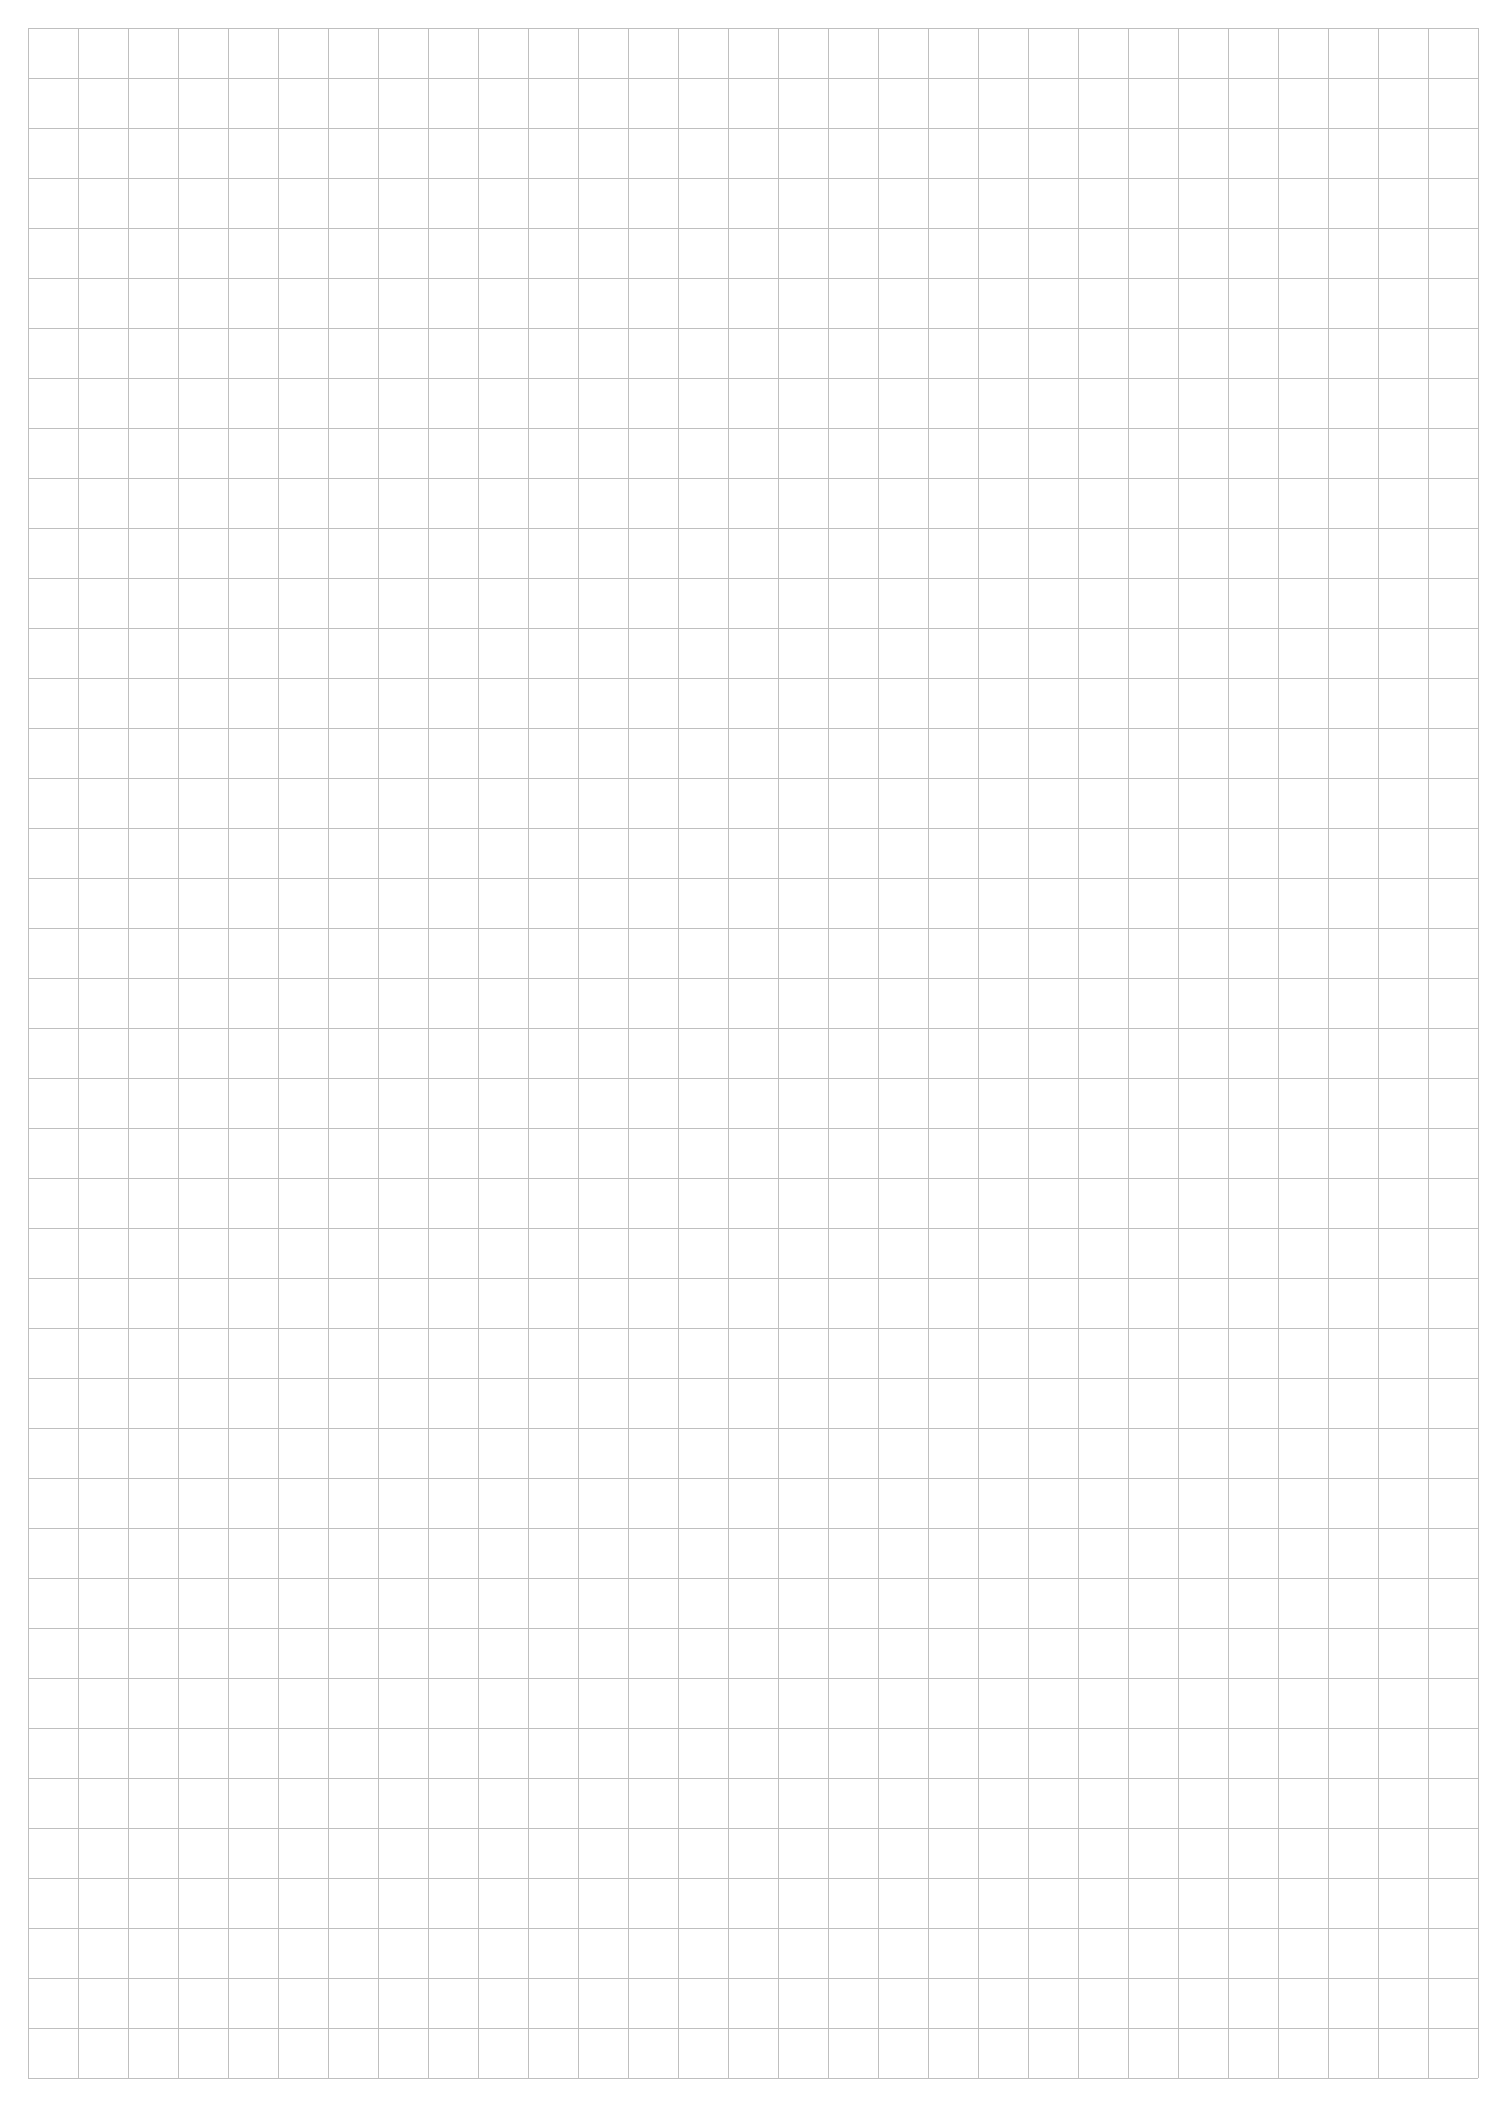
\begin{tikzpicture}[line width=0.1mm]
		\draw[color=gray!50, step=0.25in] (0,0) grid +(7.25in,10.25in);
	\end{tikzpicture}
\end{textblock*}


\begin{textblock*}{6.775in}(1in, 0.225in)
  \cbox{
    \centering\huge
    \textbf{Engineering Statics - 02 Force Vectors Handout}
  }
\end{textblock*}

\begin{textblock*}{4in}(1in, 1in)
	\cbox{
		\underline{Example 1} \parm
			      % A displacement is a change in position. It has a magnitude (the distance moved) and a direction, so displacement is a vector quantity.\parb
			      A truck drives due east on a straight road for 40 km, then drives north on a straight road for 30 km before stopping. \parb
			      What is the resultant displacement of the truck?

	}
\end{textblock*}

\begin{textblock*}{4in}(1in, 5in)
	\cbox{
		\underline{Example 2} \parm
		A plane flies NNW (i.e., $22.5\deg$ west of north) with a velocity of $275\text{ km/h}$. There is a wind blowing at $55\text{ km/h}$ from the NW \lb(i.e., $45\deg$ west of north).
			      \parb Determine the resultant velocity of the plane relative to the ground.
			      \parb Determine the wind speed that would cause the plane to fly due north. What is the ground speed in this case?

	}
\end{textblock*}
%%%%%%%%%%%%%%%%%%%%%%%%%%%%%%%%%%%%%%%%%%%%%%%%%%%%%%%%%%%%%%%%%%%%%%%%%%%%%%%%%%%%%%%%%%%%%%%%%%%%
% page 2
%%%%%%%%%%%%%%%%%%%%%%%%%%%%%%%%%%%%%%%%%%%%%%%%%%%%%%%%%%%%%%%%%%%%%%%%%%%%%%%%%%%%%%%%%%%%%%%%%%%%

.\newpage
\begin{textblock*}{7.25in}(1in, 0.4in)
	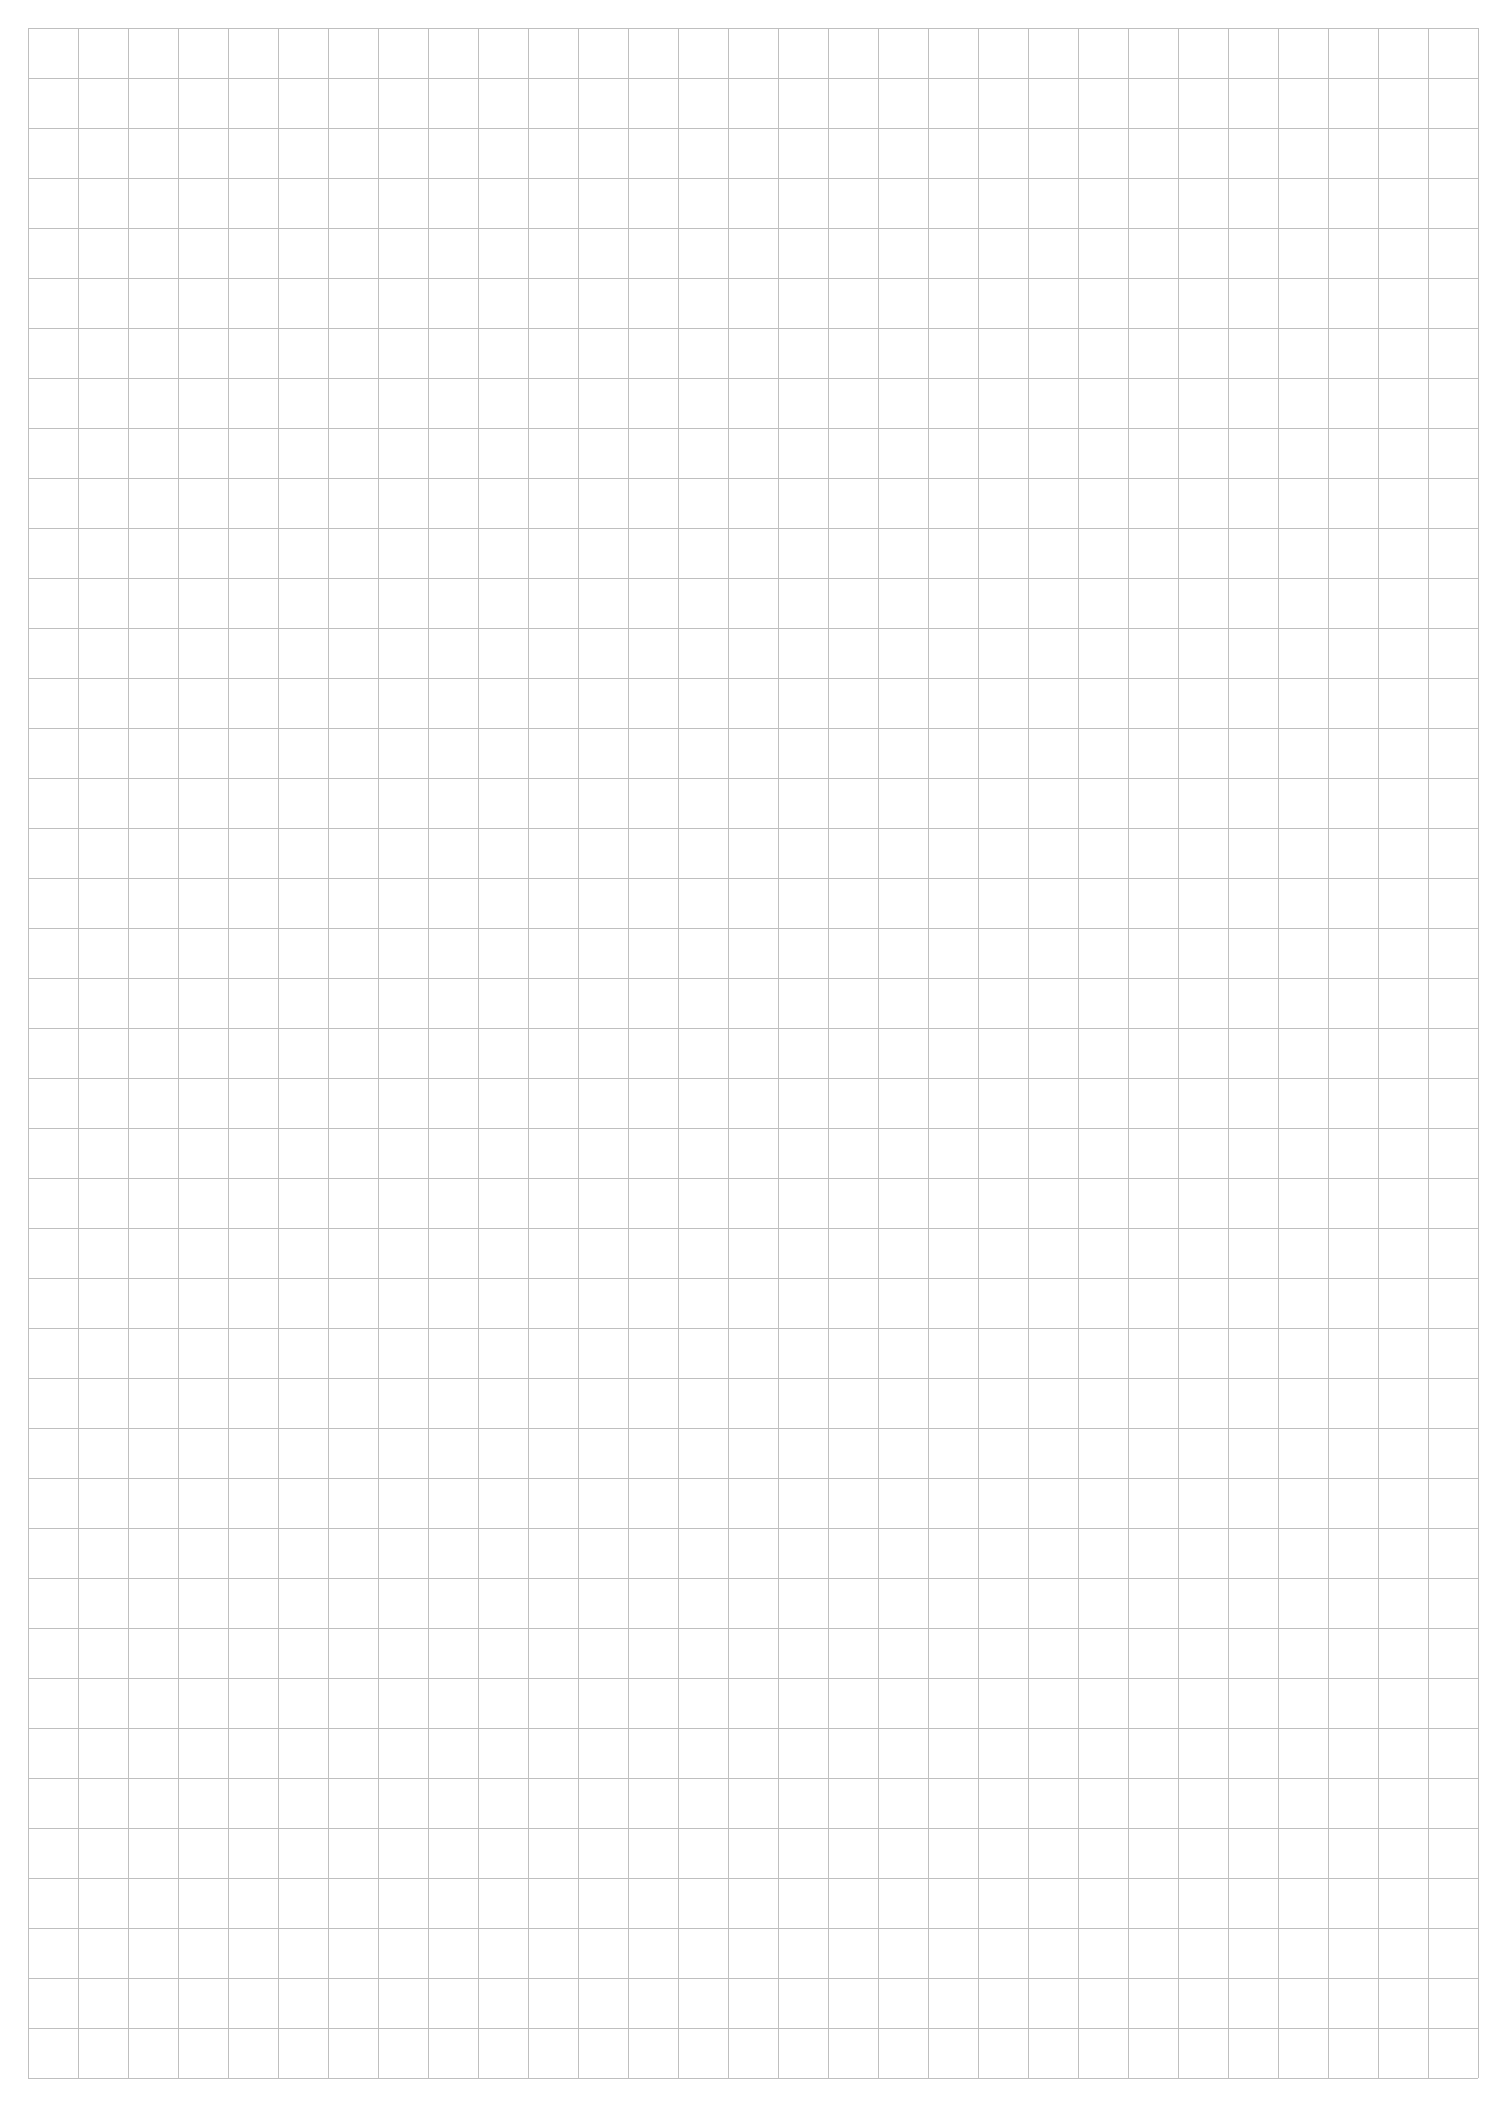
\begin{tikzpicture}[line width=0.1mm]
		\draw[color=gray!50, step=0.25in] (0,0) grid +(7.25in,10.25in);
	\end{tikzpicture}
\end{textblock*}

\begin{textblock*}{3.5in}(1in, 0.225in)
	\cbox{
		\underline{Example 3} \parm
		Determine the magnitude and the direction (measured clockwise from the the positive $x$-axis) of the resultant of the two forces.

	}
\end{textblock*}
\begin{textblock*}{2.75in}(5.03in, 0.225in)
	\def\scale{0.95}
	\cbox{
		\centering
		
		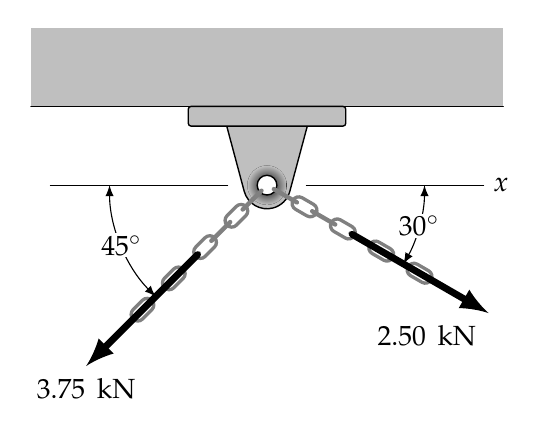
\begin{tikzpicture}[scale=\scale, line cap=round,
			postaction=decorate,
  		decoration = {markings, mark = between positions 0
  		and 1 step 16pt with 
				{
					\begin{scope}[scale=0.8]
						\draw[gray, very thick]  (0, -3pt)--++(3pt, 0)arc(-90:90:3pt)--++(-6pt,0)arc(90:270:3pt)--cycle;
						\draw[gray,ultra thick] (-16pt,0) -- (-4pt,0); 
					\end{scope}
				}
			}
		]

	\coordinate (D) at (-3,1);
	\coordinate (E) at (3, 2);
	\coordinate (C) at (0, 0);

	\fill[gray!50] (D) rectangle (E);
	\draw[thin, black] (D) -- ($(E)-(0,1) $);
	\EyeConnection[180]{C}{gray!50}{black}{1}{0.5};

	\draw[latex-latex] ($ (C)+(180:2)$) arc (180:225:2) node[fill=white, midway, inner sep=0.25mm] {$ 45\deg $};
	\draw[latex-latex] ($ (C)+(0:2)$) arc (0:-30:2) node[fill=white, midway, inner sep=0.25mm] {$ 30\deg $};


	\path[postaction={decorate}] ($ (C)+(-30:0.55) $) -- +(-30:2);
	\path[postaction={decorate}] ($ (C)+(225:0.55) $) -- +(225:2);
	\draw[line width=0.875mm, -latex] ($ (C)+(-30:1.25) $) -- +(-30:2) node[black, below left]{\(2.50\,\text{ kN}\)};
	\draw[line width=0.875mm, -latex] ($ (C)+(225:1.25) $) -- +(225:2) node[black, below]{\(3.75\,\text{ kN}\)};

	\draw[thin] ($(C)+(-0.5,0) $) -- +(-2.25,0);
	\draw[thin] ($(C)+(0.5,0) $) -- +(2.25,0) node[right] {$x$};



	


\end{tikzpicture}
	}
\end{textblock*}

\begin{textblock*}{3in}(1in, 5in)
	\cbox{
		\underline{Exercise 1} \parm
		The resultant of the forces $F$ and $F_1$ is $3.14$ kN at $37^\circ$ clockwise from the
					positive $x$ axis.\parm
					Determine $F$ and $\theta$.

	}
\end{textblock*}
\begin{textblock*}{3.25in}(4.525in, 5in)
	\cbox{
		\centering
		\def\scale{0.8}
		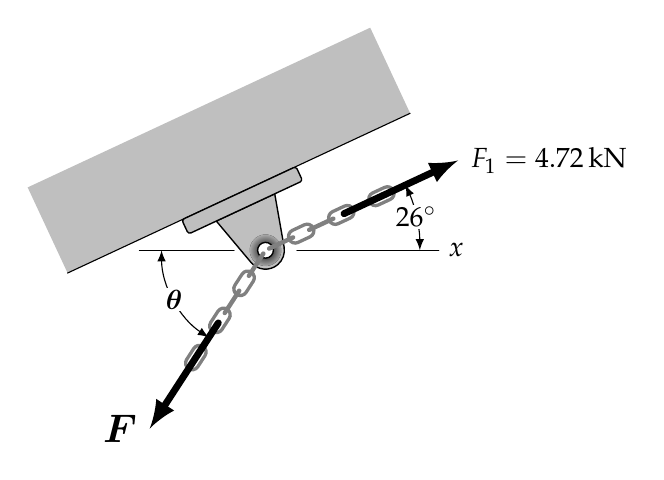
\begin{tikzpicture}[scale=0.8, line cap=round,
			postaction=decorate,
  		decoration = {markings, mark = between positions 0
  		and 1 step 16pt with 
				{
					\begin{scope}[scale=0.8]
						\draw[gray, very thick]  (0, -3pt)--++(3pt, 0)arc(-90:90:3pt)--++(-6pt,0)arc(90:270:3pt)--cycle;
						\draw[gray,ultra thick] (-16pt,0) -- (-4pt,0); 
					\end{scope}
				}
			}
		]

	\coordinate (D) at (-3,1);
	\coordinate (E) at (3, 2.5);
	\coordinate (C) at (0, 0);

\begin{scope}[rotate=25]
	\fill[gray!50] (-3,1) rectangle (3,2.5);
	\draw[thin, black] (-3,1) -- ($(3,2.5)-(0,1.5)$);
	\EyeConnection[180]{C}{gray!50}{black}{1}{0.5}
\end{scope}

	\draw[latex-latex] ($(C)+(180:1.65)$) arc (180:237:1.65) node[fill=white, midway, inner sep=0.25mm] {$\bm \theta$};
	\draw[latex-latex] ($(C)+(0:2.45)$) arc (0:25:2.45) node[fill=white, midway, inner sep=0.25mm] {$ 26^\circ $};


	\path[postaction={decorate}] ($(C)+(25:0.625)$) -- +(25:2);
	\path[postaction={decorate}] ($(C)+(237:0.625)$) -- +(237:2);
	\draw[line width=0.875mm, -latex] ($(C)+(25:1.375)$) -- +(25:2) node[black, right]{$F_1=4.72\,\mathrm{kN}$};
	\draw[line width=0.875mm, -latex] ($(C)+(237:1.375)$) -- +(237:2) node[left]{\Large $\bm F $};

	\draw[thin] ($(C)+(-0.5,0)$) -- +(-1.5,0);
	\draw[thin] ($(C)+(0.5,0)$) -- +(2.25,0) node[right] {$x$};




\end{tikzpicture}

	}
\end{textblock*}



%%%%%%%%%%%%%%%%%%%%%%%%%%%%%%%%%%%%%%%%%%%%%%%%%%%%%%%%%%%%%%%%%%%%%%%%%%%%%%%%%%%%%%%%%%%%%%%%%%%%
% page 3
%%%%%%%%%%%%%%%%%%%%%%%%%%%%%%%%%%%%%%%%%%%%%%%%%%%%%%%%%%%%%%%%%%%%%%%%%%%%%%%%%%%%%%%%%%%%%%%%%%%%
.\newpage
\begin{textblock*}{7.25in}(1in, 0.4in)
  % \textblockcolor{pink}
	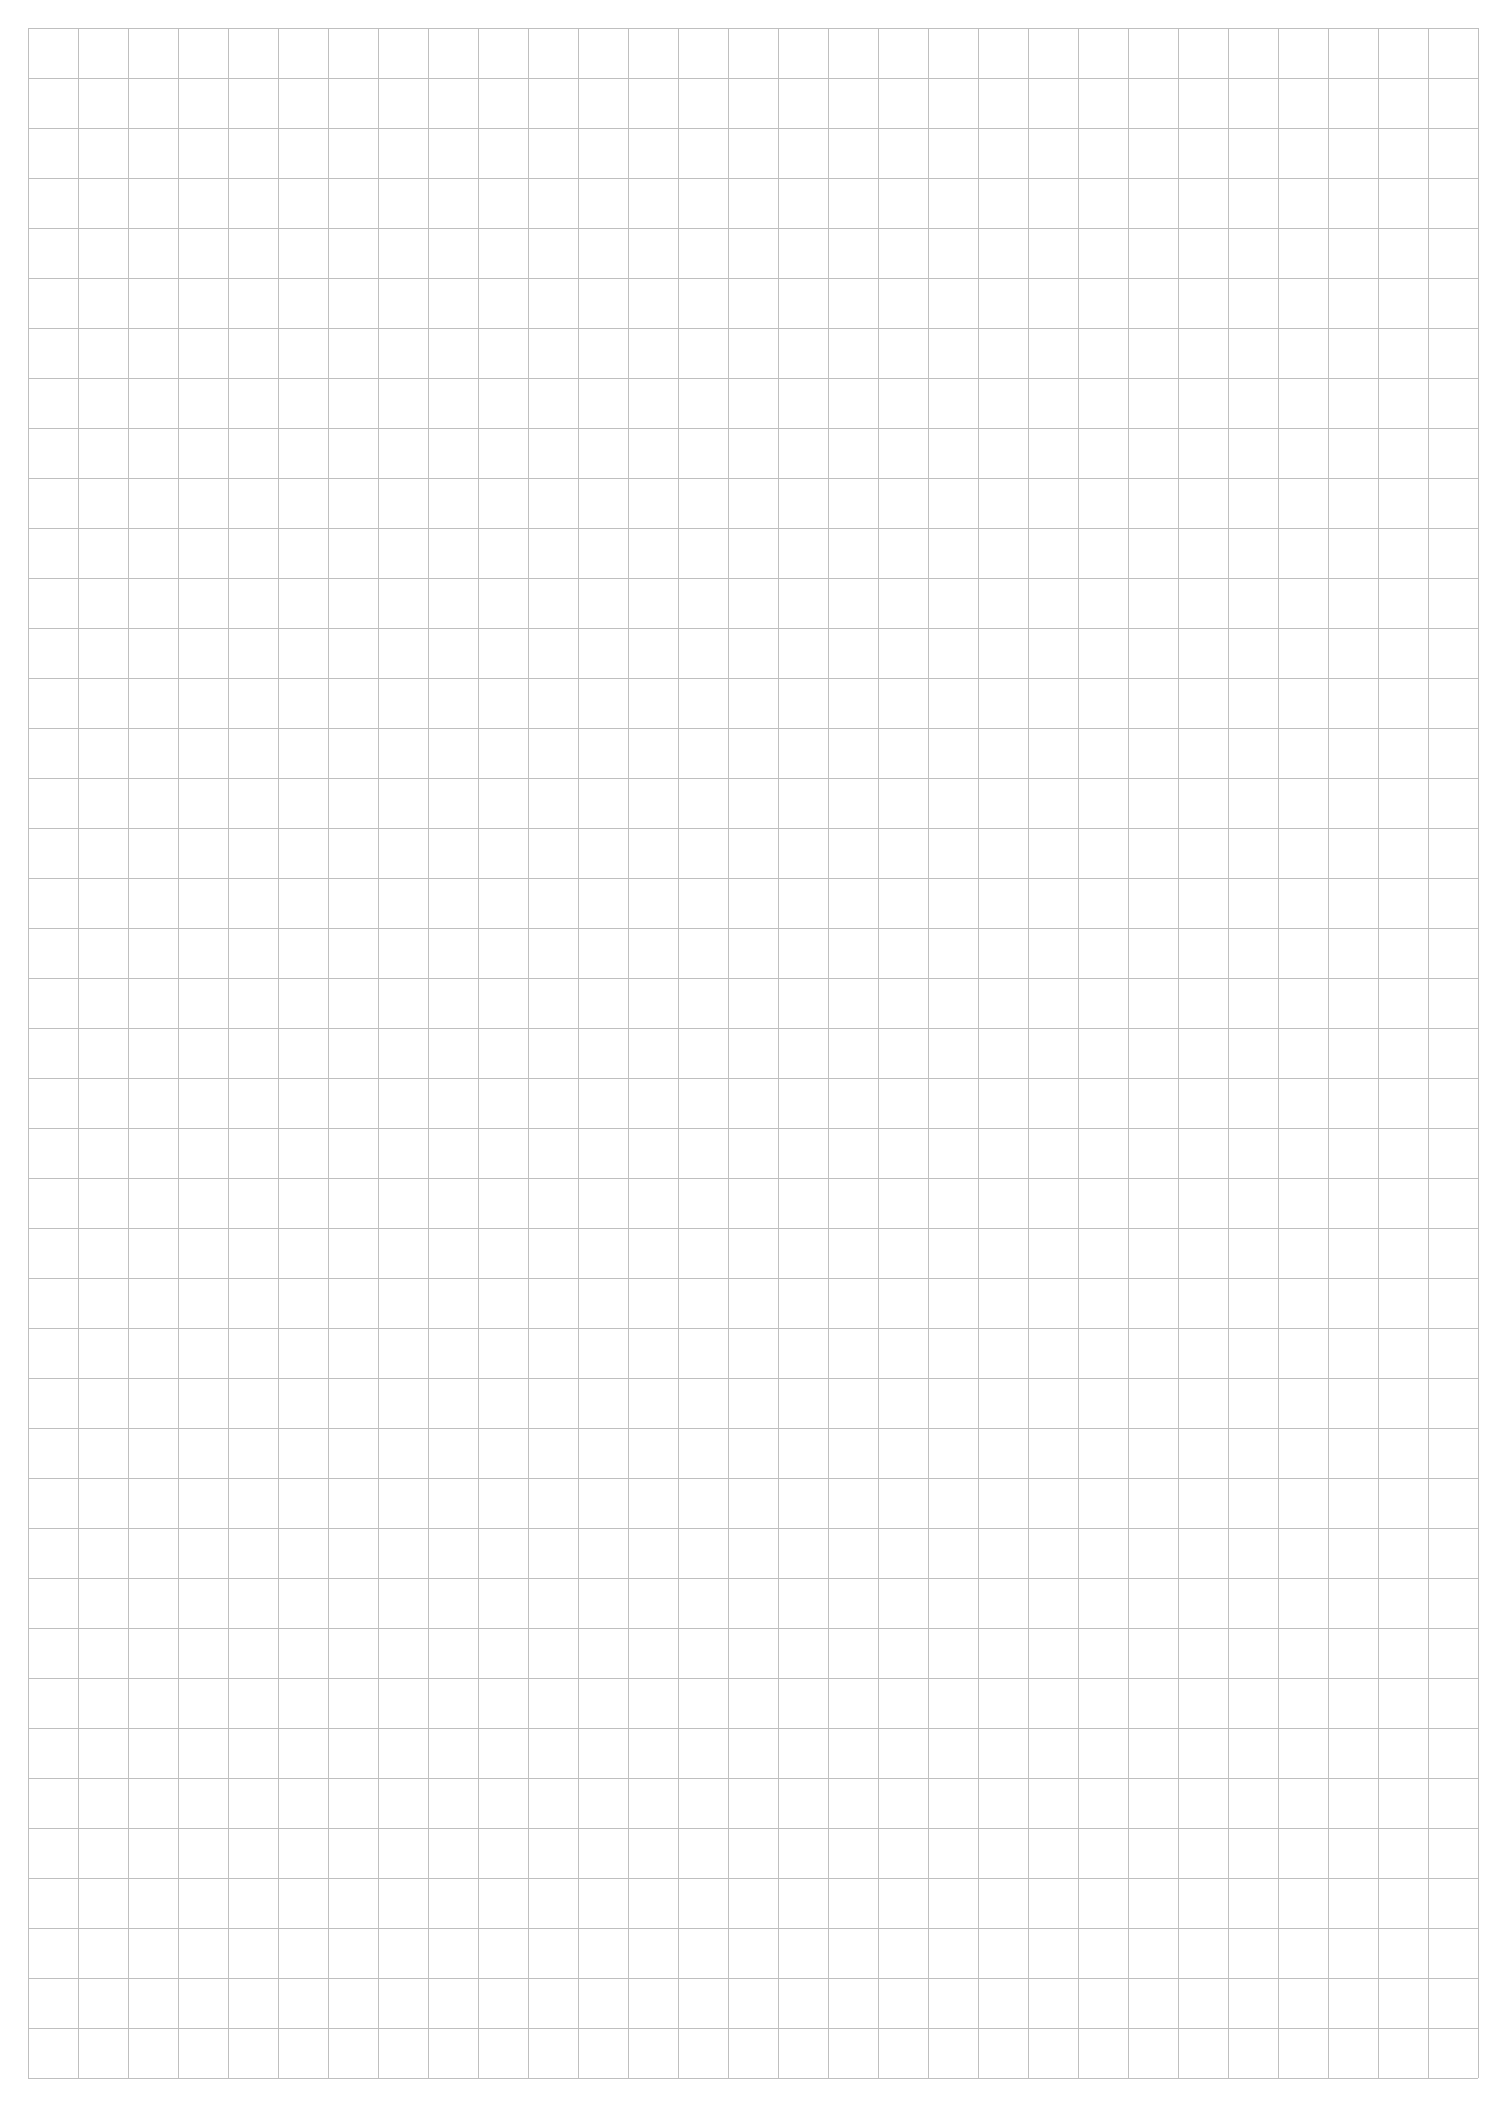
\begin{tikzpicture}[line width=0.1mm]
		\draw[color=gray!50, step=0.25in] (0,0) grid +(7.25in,10.25in);
	\end{tikzpicture}
\end{textblock*}

\begin{textblock*}{4in}(1in, 0in)
	\cbox{
		\underline{Example 4} \parm
		The weight, $W$, of the traffic lights (with mass $105\;\text{kg}$) acts vertically downward.
					\parm
					Find the value of $ W$ and use it to determine the magnitudes of its two components directed along the axes of $AC$ and $BC$.

	}
\end{textblock*}
\begin{textblock*}{2.25in}(5.525in, 0in)
	\cbox{
		\centering
		\scalebox{1.25}{
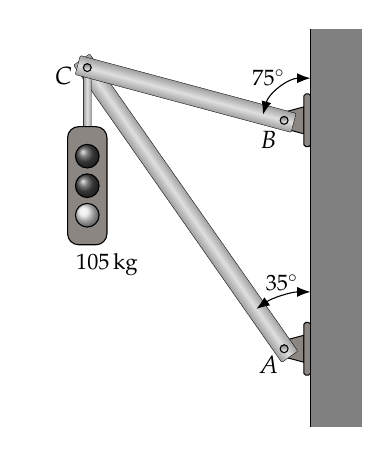
\begin{tikzpicture}[scale=0.5]

	\coordinate (C) at (0,0);
	\coordinate (B) at ($ (C)+(-15:5.176) $);
	\coordinate (A) at ($ (C)+(-55:8.717) $);
	\coordinate (D) at ($ (C)+(0,-3) $);

	\gettikzxy{(A)}{\ax}{\ay}
  \gettikzxy{(B)}{\bx}{\by}
  \gettikzxy{(C)}{\cx}{\cy}

	\PC[90]{B}{Seashell4}{black}{0.67}{0.125}
	\PC[90]{A}{Seashell4}{black}{0.67}{0.125}

	\fill[gray] ($ (\bx+0.67cm, \cy+1cm) $) rectangle ($ (\ax+2cm, \ay-2cm) $);
	\draw[thin]  ($ (\bx+0.67cm, \cy+1cm) $) -- ($ (\bx+0.67cm, \ay-2cm) $);
	
	\Member{C}{A}{gray!75!white}{gray!25!white}{black}{0.5}{.125}{0.125}	
	\Member{C}{D}{gray!75!white}{gray!25!white}{black}{0.2}{.1}{0.125}
	\Member{C}{B}{gray!75!white}{gray!25!white}{black}{0.5}{.125}{0.125}

	\filldraw[rounded corners, fill=Seashell4] ($ (D)+(-0.5,-1.5) $) rectangle ($ (D)+(0.5,1.5) $);
	\shadedraw[ball color=gray!60!black] (D) circle (.3cm);
	\shadedraw[ball color=gray!60!black] ($(D)+(0,0.75)$) circle (.3cm);
	\shadedraw[ball color=gray!20] ($(D)+(0,-0.75)$) circle (.3cm);
	\node at ($ (D)-(-0.5,2) $) {\footnotesize $ 105\,$kg};

	\draw[Latex-Latex] ($ (B)+(-15:0.6936)+(0,1.25) $) arc (90:165:1.25) node[midway,xshift=-1.5mm, yshift=1.3mm] {\footnotesize $75\deg$};
	\draw[Latex-Latex] ($ (A)+(-55:1.168)+(0,2.4) $) arc (90:125:2.4) node[midway,yshift=1.75mm] {\footnotesize $35\deg$};

	\small
	
	\shadedraw [draw=black] (B) circle (0.1cm) node[xshift=-0.2cm, yshift=-0.25cm] {$B$};
	\shadedraw [draw=black] (A) circle (0.1cm) node[xshift=-0.2cm, yshift=-0.2cm] {$A$};
	\shadedraw [draw=black] (C) circle (0.1cm) node[xshift=-0.3cm, yshift=-0.1cm] {$C$};

	\pgfresetboundingbox
	\draw[white] (\cx-1.5cm, \cy+1cm) rectangle (\ax+2cm, \ay-2cm);
	

\end{tikzpicture}


}
		
	}
\end{textblock*}

\begin{textblock*}{2.5in}(1in, 5in)
	\cbox{
	\underline{Exercise 2} \parm
		Resolve the $4.20$ kN load suspended from $A$ into components parallel to the truss members $AB$ and $AG$.
		\parm
		Give the magnitude of the components and their direction measured counter-clockwise from the positive $x$ axis.

	}
\end{textblock*}
\begin{textblock*}{3.75in}(4.025in, 5in)
	\cbox{
		\centering
		\scalebox{0.8}{
			\tikz{%
  \coordinate (A) at (0,0);
  \coordinate (B) at (2.5,0);
  \coordinate (C) at (5.5,0);
  \coordinate (D) at (8,1.25);
  \coordinate (E) at (8,-3);
  \coordinate (F) at (5.5,-3);
  \coordinate (G) at (2.5,-3);

  \gettikzxy{(C)}{\Cx}{\Cy};
	\gettikzxy{(E)}{\Ex}{\Ey};
	\gettikzxy{(D)}{\Dx}{\Dy};

  \fill[gray] ($ (E)+(0.5,-1) $) rectangle ($ (D)+(1.5,1.5) $);
	\draw[black, thick] ($ (E)+(0.5,-1) $) -- ($ (D)+(0.5,1.5) $);

  \PC[90]{D}{gray}{black}{0.5}{0.25}
	\PC[90]{E}{gray}{black}{0.5}{0.25}

  \Member{A}{B}{gray}{white}{black}{0.3125}{0.15}{0.125}
  \Member{B}{C}{gray}{white}{black}{0.3125}{0.15}{0.125}
  \Member{C}{D}{gray}{white}{black}{0.3125}{0.15}{0.125}
  \Member{E}{F}{gray}{white}{black}{0.3125}{0.15}{0.125}
  \Member{F}{G}{gray}{white}{black}{0.3125}{0.15}{0.125}
  \Member{A}{G}{gray}{white}{black}{0.3125}{0.15}{0.125}
  \Member{C}{G}{gray}{white}{black}{0.3125}{0.15}{0.125}
  \Member{C}{E}{gray}{white}{black}{0.3125}{0.15}{0.125}
  \Member{B}{G}{gray}{white}{black}{0.3125}{0.15}{0.125}
  \Member{C}{F}{gray}{white}{black}{0.3125}{0.15}{0.125}

  \draw[thin, black] ($ (A)+(0,0.325)$) -- +(0,2.25);
  \draw[thin, black] ($ (B)+(0,0.325)$) -- +(0,2.25);
  \draw[thin, black] ($ (C)+(0,0.325)$) -- +(0,2.25);
  \draw[thin, black] ($ (D)+(0,0.325)$) -- +(0,1);
  \draw[thin, black] ($ (D)+(0.25,0)$) -- +(2.25,0);
  \draw[thin, black] ($ (E)+(0.25,0)$) -- +(2.25,0);
  \draw[thin, black] ($ (C)+(0.5,0)$) -- +(4.5,0);

  \draw[thick, latex-latex] ([yshift=2.125cm]A) -- node[fill=white, inner sep=0.375mm]{$2.50$ m}([yshift=2.125cm]B);
	\draw[thick, latex-latex] ([yshift=2.125cm]B) -- node[fill=white, inner sep=0.375mm]{$3.00$ m}([yshift=2.125cm]C);
	\draw[thick, latex-latex] ([yshift=2.125cm]C) -- node[fill=white, inner sep=0.375mm]{$2.50$ m}([yshift=0.875cm]D);
	\draw[thick, latex-latex] (10.125, \Dy) -- node[fill=white, inner sep=0.75mm]{$1.25$ m}(10.125, \Cy);
	\draw[thick, latex-latex] (10.125, \Cy) -- node[fill=white, inner sep=0.75mm]{$3.00$ m}(10.125, \Ey);


  \draw[line width=0.625mm, -Latex, line cap=round] (A) -- +(0,-2.5) node[below] {\Large {$\bm{4.20}$ \bf kN}};

  \fill[ball color=gray] (A) circle (3pt) node[above left, inner sep=2mm] {\large $\bm A$};
	\fill[ball color=gray] (B) circle (3pt) node[above left, inner sep=2mm] {\large $\bm B$};
	\fill[ball color=gray] (C) circle (3pt) node[above left, inner sep=2mm] {\large $\bm C$};
	\fill[ball color=gray] (D) circle (3pt) node[above left, inner sep=1.5mm] {\large $\bm D$};
	\fill[ball color=gray] (E) circle (3pt) node[below left, inner sep=2.5mm] {\large $\bm E$};
	\fill[ball color=gray] (F) circle (3pt) node[below left, inner sep=2mm] {\large $\bm F$};
	\fill[ball color=gray] (G) circle (3pt) node[below left, inner sep=2mm] {\large $\bm G$};


  % \pgfresetboundingbox
  \useasboundingbox ($ (A)+ (-0.75,3) $) rectangle ($ (E)+(2.875,-1.25) $);





}
		}
	}
\end{textblock*}




%%%%%%%%%%%%%%%%%%%%%%%%%%%%%%%%%%%%%%%%%%%%%%%%%%%%%%%%%%%%%%%%%%%%%%%%%%%%%%%%%%%%%%%%%%%%%%%%%%%%
% page 4
%%%%%%%%%%%%%%%%%%%%%%%%%%%%%%%%%%%%%%%%%%%%%%%%%%%%%%%%%%%%%%%%%%%%%%%%%%%%%%%%%%%%%%%%%%%%%%%%%%%%
.\newpage
\begin{textblock*}{7.25in}(1in, 0.375in)
	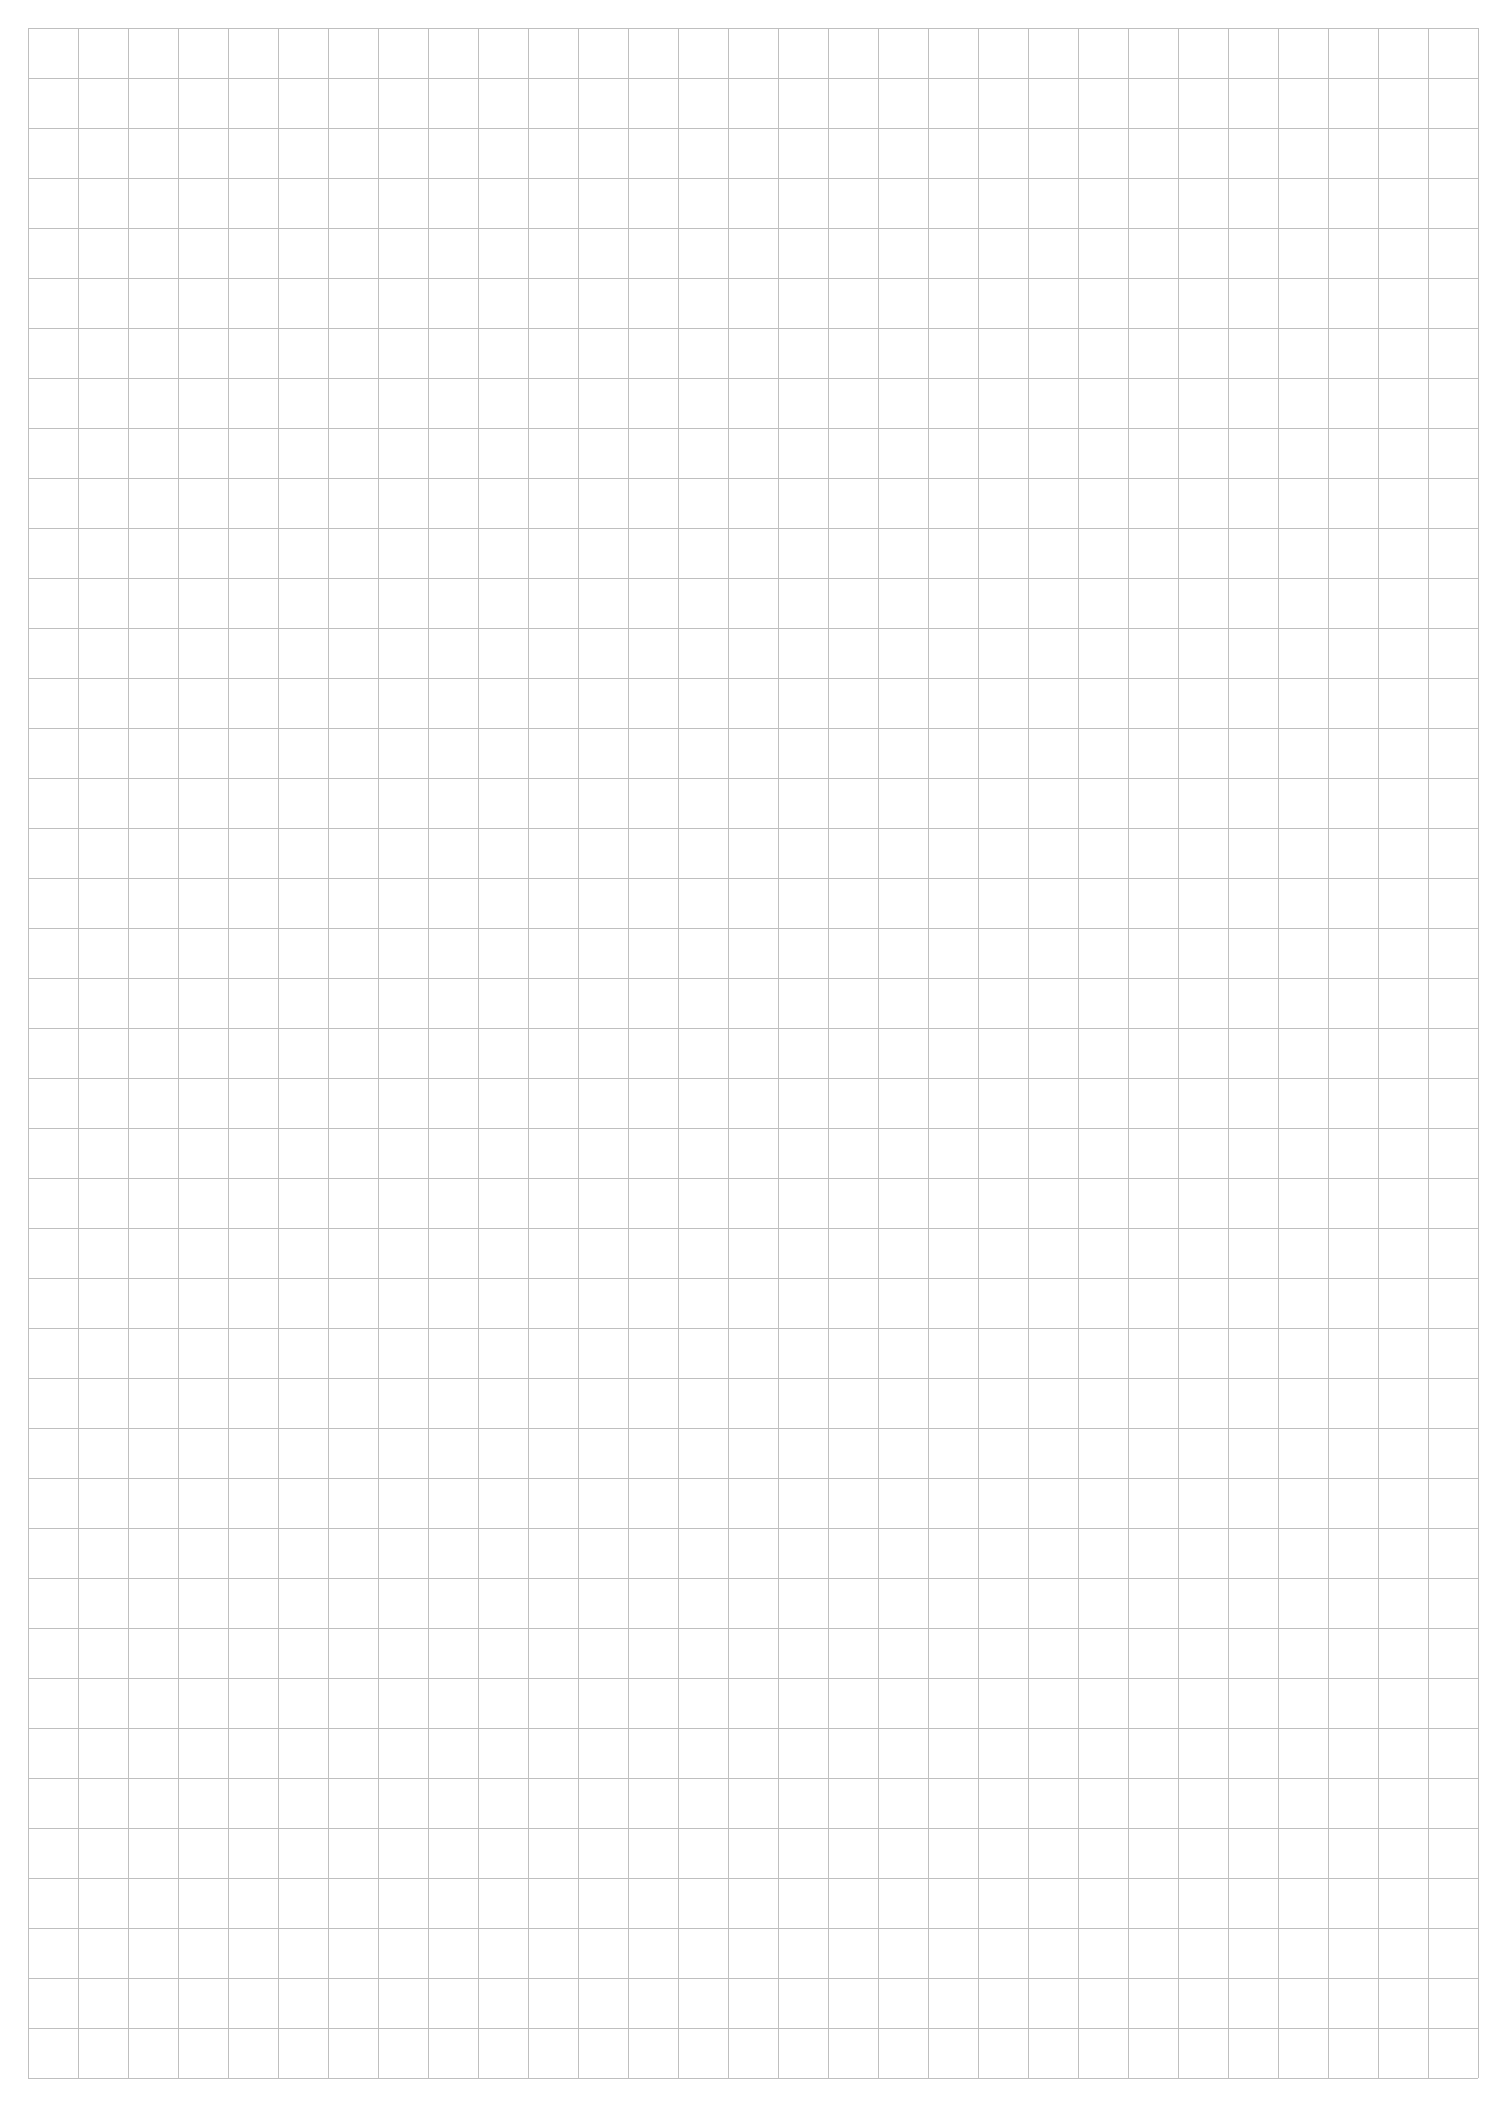
\begin{tikzpicture}[line width=0.1mm]
		\draw[color=gray!50, step=0.25in] (0,0) grid +(7.25in,10.25in);
	\end{tikzpicture}
\end{textblock*}

\begin{textblock*}{3.75in}(1in, 0.235in)
	\cbox{
		\underline{Exercise 3} \parm
		The decoration suspended at $D$ weighs $1124\,\mathsf{N}$.\parm 
				Determine the magnitudes of the two force components of the weight of $D$, in the direction of $AB$ and $BC$.

	}
\end{textblock*}
\begin{textblock*}{2.5in}(5.275in, 0.235in)
	\cbox{
		\centering
		\def\scale{0.8}
		
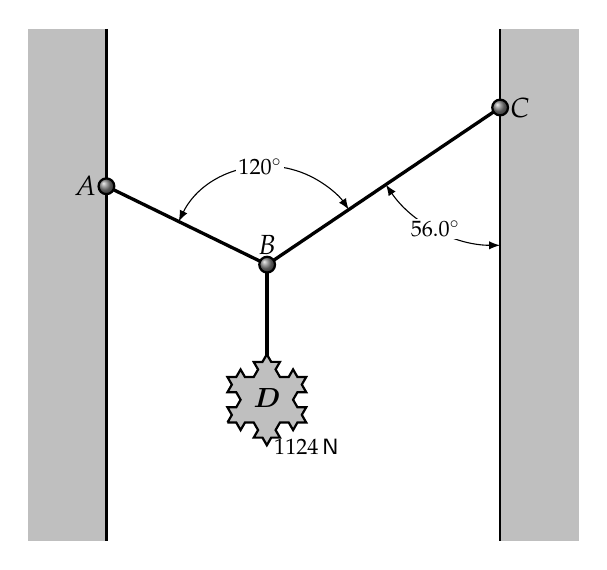
\begin{tikzpicture}[scale=\scale, decoration=Koch snowflake,fill=gray!50,thick]

	\coordinate (A) at (0,-2);
	\coordinate (AA) at ($(A)+(-26:1)$);
	\coordinate (C) at (5,-1);
	\coordinate (CC) at ($(C)+(214:1)$);
	\coordinate (B) at (intersection of A--AA and C--CC);
	\coordinate (D) at ($ (B)+(0,-1.6875) $);

	\fill[gray!50] ($ (A)+(0,2) $) rectangle  ($ (A)+(-1,-4.5) $); 
	\fill[gray!50] ($ (C)+(0,1) $) rectangle  ($ (C)+(1,-5.5) $); 
	\draw[thick] ($ (A)+(0,2) $) -- ($ (A)+(0,-4.5) $); 
	\draw[thick] ($ (C)+(0,1) $) -- ($ (C)+(0,-5.5) $); 


	\draw[very thick] (A)--(B);
	\draw[very thick] (B)--(C);
	\draw[very thick] (B)--(D);

	\filldraw[xshift=1.5375cm, yshift=-2.5cm] decorate{ decorate{ (0,-2.5) -- ++(60:1) -- ++(-60:1) -- cycle }};


	\draw[thin, latex-latex] ($ (B)+(154:1.25) $) arc (154:34:1.25) node[fill=white, inner sep=0.25mm, midway] {\footnotesize $120\deg$};
	\draw[thin, latex-latex] ($ (C)+(270:1.75) $) arc (270:214:1.75) node[fill=white, inner sep=0.25mm, midway] {\footnotesize $56.0\deg$};


	\shadedraw [draw=black, ball color = gray] (B) circle (0.1cm) node[above] {$B$};
	\shadedraw [draw=black, ball color = gray] (A) circle (0.1cm) node[left] {$A$};
	\shadedraw [draw=black, ball color = gray] (C) circle (0.1cm) node[right] {$C$};
	\node at (D) {$\bm D$};
	\node[black, xshift=0.5cm, yshift=-0.625cm] at (D) {\footnotesize $1124\,\mathsf{N}$};



\end{tikzpicture}

	}
\end{textblock*}

\begin{textblock*}{4.25in}(1in, 5.25in)
	\cbox{
	\underline{Example 5} \parm
	\begin{enumerate}[{a)}]
		\item Determine the resultant $\bm R $ of the two vectors $\bm F$ and $\bm G $.
		\item Determine the $x$-component of $\bm R$ \lb(i.e., the horizontal component).
		% \item Determine the $y$-component of ${\bm{\mathrm{ R }}}$ \lb(i.e., the vertical component).
		\item Determine the $x$-component of $\bm F$.
		\item Determine the $x$-component of $\bm G$.
		\item Add the two previous results.
	\end{enumerate}

	}
\end{textblock*}
\begin{textblock*}{2in}(5.765in, 5.25in)
	\cbox{
		\centering
		
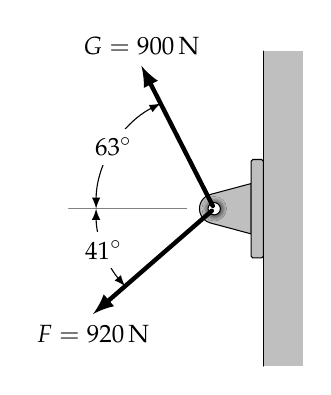
\begin{tikzpicture}[scale=\scale, line cap = round]

	\coordinate (A) at (0,0);

	\EyeConnection[90]{A}{gray!50}{black}{0.625}{0.375}
	\fill[gray!50] ($ (A)+(0.625,2) $) rectangle ($ (A)+(1.125,-2) $);
	\draw ($ (A)+(0.625,2) $) -- ($ (A)+(0.625,-2) $);

	\draw[ultra thick, -latex] ($ (A)+(117:0.04) $) -- +(117:2) node[black, yshift=0.25cm] {\small $ G=900\,$N};
	\draw[ultra thick, -latex] ($ (A)+(221:0.04) $) -- +(221:2) node[black, yshift=-0.25cm] {\small $ F=920\,$N};

	\draw[gray] ($ (A)-(0.35cm,0) $) -- +(-1.5,0);

	\draw[latex-latex] ($ (A)+(117:1.5) $) arc (117:180:1.5) node[midway, fill=white] {\small $ 63\deg $};
	\draw[latex-latex] ($ (A)+(221:1.5) $) arc (221:180:1.5) node[midway, fill=white] {\small $ 41\deg $};


\end{tikzpicture}

	}
\end{textblock*}


%%%%%%%%%%%%%%%%%%%%%%%%%%%%%%%%%%%%%%%%%%%%%%%%%%%%%%%%%%%%%%%%%%%%%%%%%%%%%%%%%%%%%%%%%%%%%%%%%%%%
% page 5
%%%%%%%%%%%%%%%%%%%%%%%%%%%%%%%%%%%%%%%%%%%%%%%%%%%%%%%%%%%%%%%%%%%%%%%%%%%%%%%%%%%%%%%%%%%%%%%%%%%%
.\newpage
\begin{textblock*}{7.25in}(1in, 0.375in)
	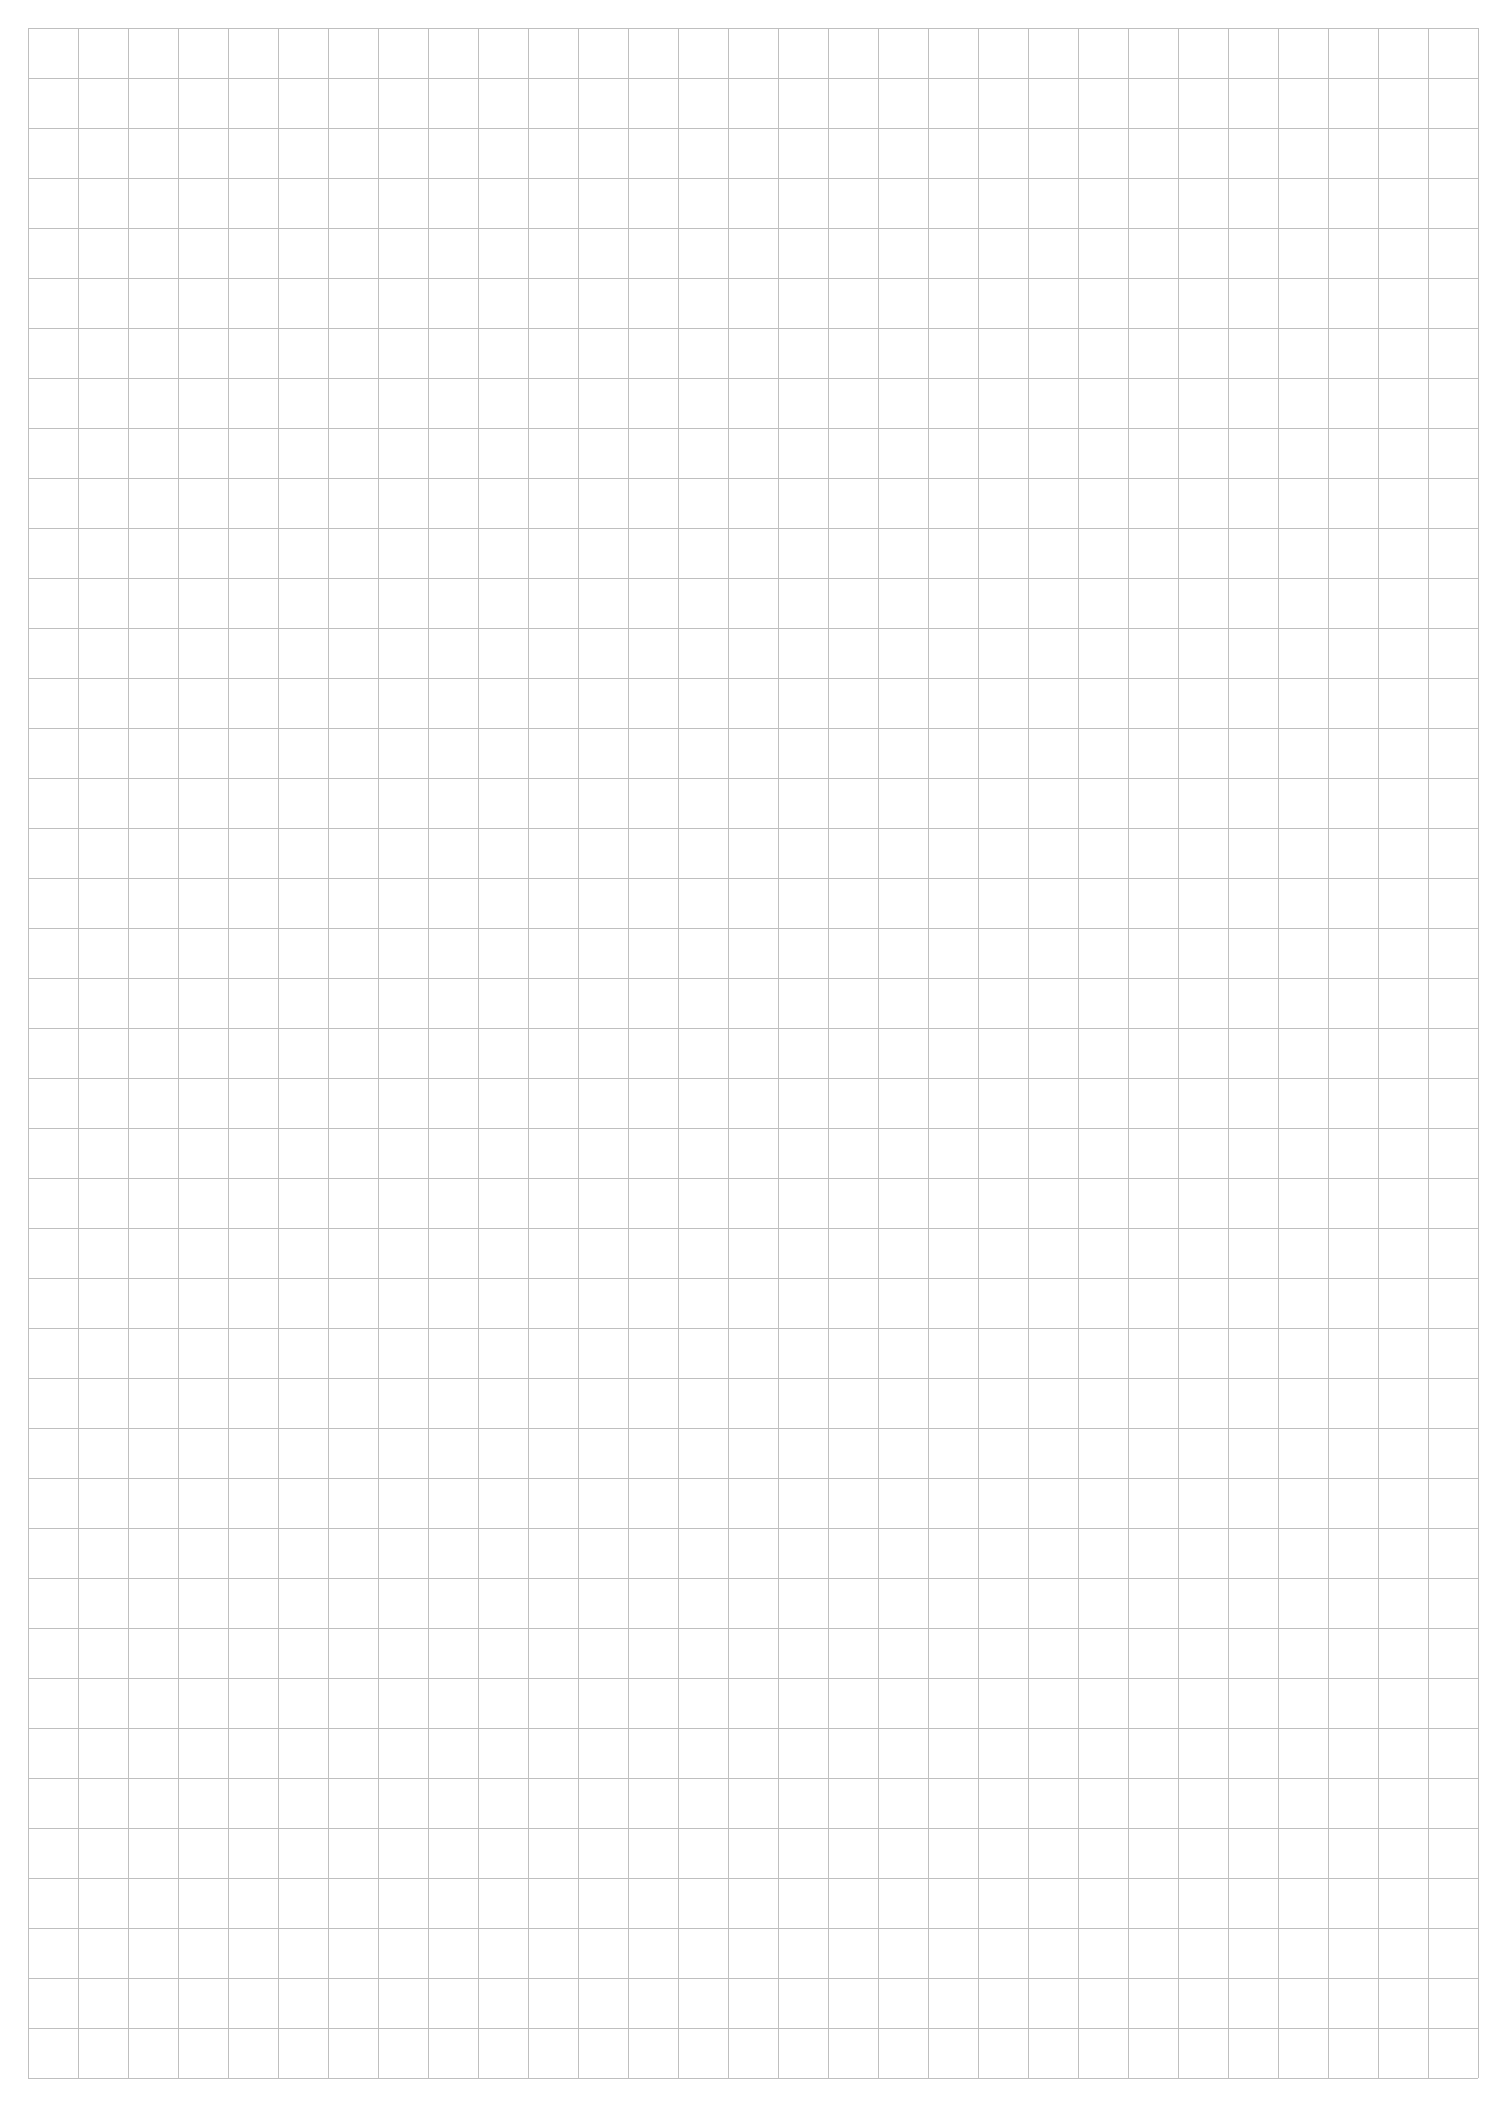
\begin{tikzpicture}[line width=0.1mm]
		\draw[color=gray!50, step=0.25in] (0,0) grid +(7.25in,10.25in);
	\end{tikzpicture}
\end{textblock*}

\begin{textblock*}{4.25in}(1in, 0.235in)
	\cbox{
		\underline{Exercise 4} \parm
		\begin{enumerate}[{a)}]
			\item Determine the magnitude of the component of ${\bm{\mathrm{ R }_{}}}$  along the $y$ axis (i.e., the vertical component).
			\item Determine the magnitude of the component of ${\bm{\mathrm{ F }_{}}}$ along the $y$ axis.
			\item Determine the magnitude of the component of ${\bm{\mathrm{ G }_{}}}$ along the $y$ axis.
			\item Add the two previous results.
		\end{enumerate}

	}
\end{textblock*}
\begin{textblock*}{2in}(5.765in, 0.235in)
	\cbox{
		\centering
		
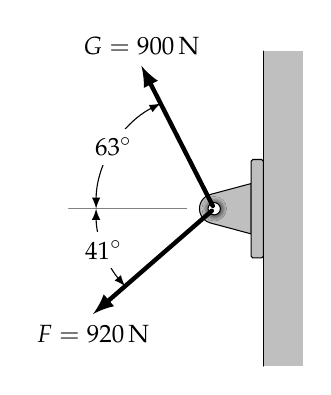
\begin{tikzpicture}[scale=\scale, line cap = round]

	\coordinate (A) at (0,0);

	\EyeConnection[90]{A}{gray!50}{black}{0.625}{0.375}
	\fill[gray!50] ($ (A)+(0.625,2) $) rectangle ($ (A)+(1.125,-2) $);
	\draw ($ (A)+(0.625,2) $) -- ($ (A)+(0.625,-2) $);

	\draw[ultra thick, -latex] ($ (A)+(117:0.04) $) -- +(117:2) node[black, yshift=0.25cm] {\small $ G=900\,$N};
	\draw[ultra thick, -latex] ($ (A)+(221:0.04) $) -- +(221:2) node[black, yshift=-0.25cm] {\small $ F=920\,$N};

	\draw[gray] ($ (A)-(0.35cm,0) $) -- +(-1.5,0);

	\draw[latex-latex] ($ (A)+(117:1.5) $) arc (117:180:1.5) node[midway, fill=white] {\small $ 63\deg $};
	\draw[latex-latex] ($ (A)+(221:1.5) $) arc (221:180:1.5) node[midway, fill=white] {\small $ 41\deg $};


\end{tikzpicture}

	}
\end{textblock*}

\begin{textblock*}{3in}(1in, 6.25in)
	\cbox{
	\underline{Example 9} \parm
		Determine the resultant (magnitude and direction counterclockwise from the positive $x$ axis) of the three forces $F_1,\;F_2$ and $F_3$ acting at a single point.

	}
\end{textblock*}
\begin{textblock*}{3.25in}(4.525in, 6.25in)
	\cbox{
	\def\scale{0.8}
	\centering
	
% !TEX root = ../../Beamer/02ForceVectors/02ForceVectors.tex


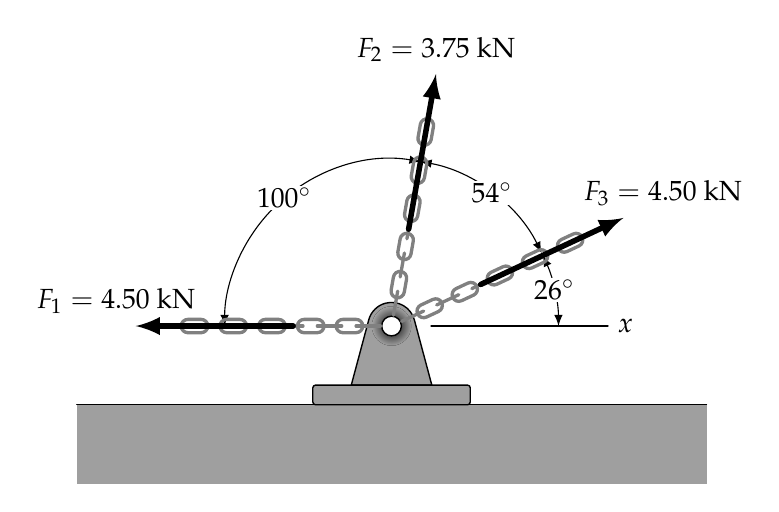
\begin{tikzpicture}[scale=\scale, line cap=round,decoration={
		markings,% switch on markings
		mark=% actually add a mark
		between positions 0 and 1 step 14pt
		with
		{
			\begin{scope}[scale=0.8]
				\draw[gray, very thick] (0pt,-3pt) -- ++(6pt,0) arc(-90:90:3pt) -- ++(-6pt,0pt) arc(90:270:3pt) -- cycle;
				\draw[gray,very thick] (-11pt,0) -- (0pt,0);
			\end{scope}
		}
	}]

	\coordinate (D) at (-3,1);
	\coordinate (E) at (3, 2.5);
	\coordinate (C) at (0, 0);

\begin{scope}
	\fill[gray!75] (-4,-1) rectangle (4,-2);
	\draw[thin, black] (-4,-1) -- ($(4,-2.5)+(0,1.5) $);
	\EyeConnection{C}{gray!75}{black}{1}{0.5}
\end{scope}

	\draw[latex-latex] ($ (C)+(26:2.12)$) arc (26:80:2.12) node[fill=white, midway, inner sep=0.25mm] {$54\deg$};
	\draw[latex-latex] ($ (C)+(0:2.12)$) arc (0:25:2.12) node[fill=white, midway, inner sep=0.25mm] {$ 26\deg $};
	\draw[latex-latex] ($ (C)+(80:2.12)$) arc (80:180:2.12) node[fill=white, midway, inner sep=0.25mm] {$ 100\deg $};


	\path[postaction={decorate}] ($ (C)+(25:0.45) $) -- +(25:2);
	\path[postaction={decorate}] ($ (C)+(180:0.45) $) -- +(180:2);
	\path[postaction={decorate}] ($ (C)+(80:0.45) $) -- +(80:2);
	\draw[line width=2pt, -latex] ($ (C)+(180:1.25) $) -- +(180:2) node[xshift=-0.25cm, black, above]{$ F_1=4.50 $ kN};
	\draw[line width=2pt, -latex] ($ (C)+(80:1.25) $) -- +(80:2) node[black, above]{$F_2=3.75 $ kN};
	\draw[line width=2pt, -latex] ($ (C)+(25:1.25) $) -- +(25:2) node[xshift=0.5cm, black, above]{$F_3=4.50 $ kN};



	\draw[thin] ($(C)+(0.5,0) $) -- +(2.25,0) node[right] {$x$};




\end{tikzpicture}

	}
\end{textblock*}


%%%%%%%%%%%%%%%%%%%%%%%%%%%%%%%%%%%%%%%%%%%%%%%%%%%%%%%%%%%%%%%%%%%%%%%%%%%%%%%%%%%%%%%%%%%%%%%%%%%%
% page 6
%%%%%%%%%%%%%%%%%%%%%%%%%%%%%%%%%%%%%%%%%%%%%%%%%%%%%%%%%%%%%%%%%%%%%%%%%%%%%%%%%%%%%%%%%%%%%%%%%%%%
.\newpage
\begin{textblock*}{7.25in}(1in, 0.375in)
	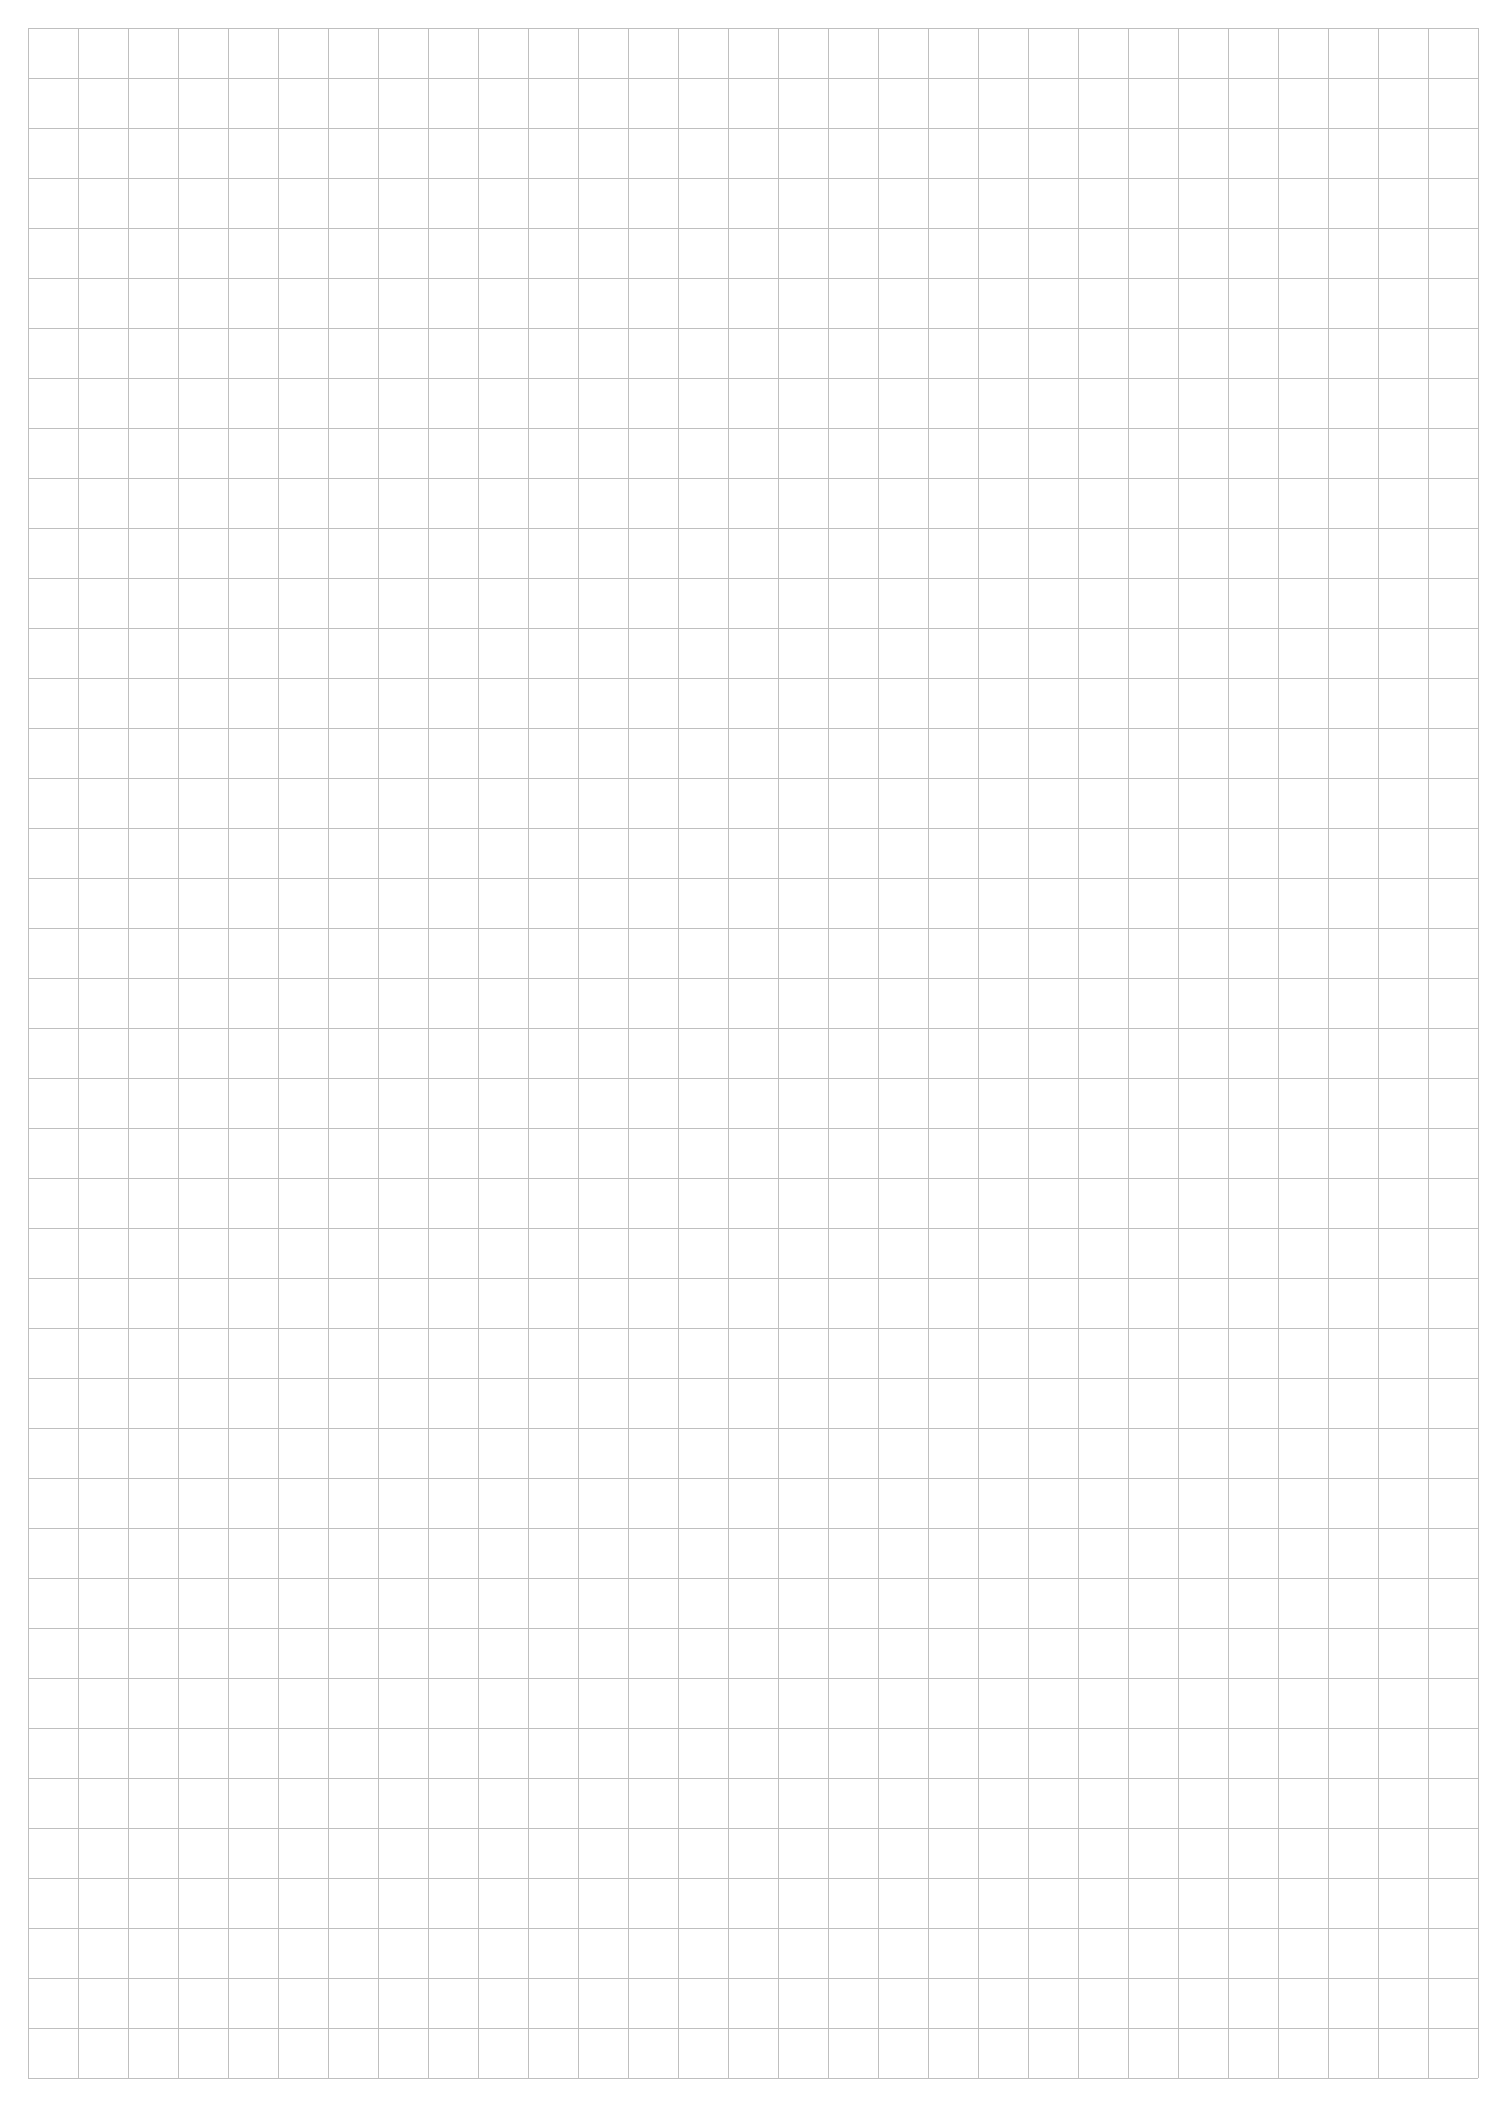
\begin{tikzpicture}[line width=0.1mm]
		\draw[color=gray!50, step=0.25in] (0,0) grid +(7.25in,10.25in);
	\end{tikzpicture}
\end{textblock*}

\begin{textblock*}{3.5in}(1in, 0.235in)
	\cbox{
		\underline{Example 10} \parm
		The resultant of the forces $F,\;F_1$ and $F_2$ acting upon the eye-bolt is $30.7$ kN at $197^\circ$ measured counter-clockwise from the positive $x$ axis. Determine $F$ and $\theta$.

	}
\end{textblock*}
\begin{textblock*}{2.75in}(5.025in, 0.235in)
	\cbox{
	\def\scale{0.8}
	\centering
	
% !TEX root = ../../Beamer/02ForceVectors/02ForceVectors.tex


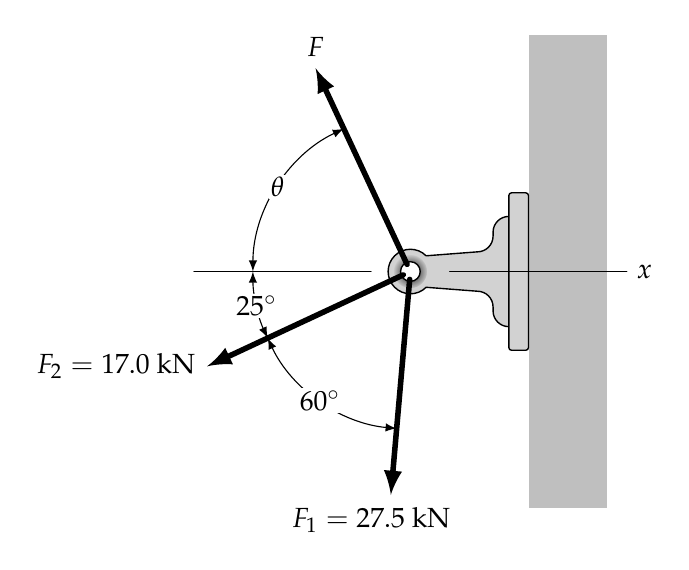
\begin{tikzpicture}[scale=\scale, line cap=round,decoration={
		markings,% switch on markings
		mark=% actually add a mark
		between positions 0 and 1 step 14pt
		with
		{
			\begin{scope}[scale=0.8]
				\draw[SteelBlue4, very thick] (0pt,-3pt) -- ++(6pt,0) arc(-90:90:3pt) -- ++(-6pt,0pt) arc(90:270:3pt) -- cycle;
				\draw[SteelBlue4,very thick] (-11pt,0) -- (0pt,0);
			\end{scope}
		}
	}]

	\coordinate (D) at (-3,1);
	\coordinate (E) at (3, 2.5);
	\coordinate (C) at (0, 0);

\begin{scope}
	\fill[gray!50] (1.5,-3) rectangle (2.5,3);
	% \draw[thin, black] (-3,-1) -- ($(3,-2.5)+(0,1.5) $);
	\EyeBolt[90]{C}{gray!35}{black}{1}{0.5}
\end{scope}

	\draw[latex-latex] ($ (C)+(115:2) $) arc (115:180:2) node[fill=white, midway, inner sep=0.25mm] {$\theta $};
	\draw[latex-latex] ($ (C)+(180:2) $) arc (180:205:2) node[fill=white, midway, inner sep=0.25mm] {$ 25^\circ $};
	\draw[latex-latex] ($ (C)+(205:2) $) arc (205:265:2) node[fill=white, midway, inner sep=0.25mm] {$ 60^\circ $};



	\draw[line width=2pt, -latex] ($ (C)+(-95:0.1) $) -- +(-95:2.75) node[xshift=-0.25cm, black, below]{$ F_1=27.5 $ kN};
	\draw[line width=2pt, -latex] ($ (C)+(115:.1) $) -- +(115:2.75) node[black, above]{$F$};
	\draw[line width=2pt, -latex] ($ (C)+(205:.1) $) -- +(205:2.75) node[black, left]{$F_2=17.0 $ kN};



	\draw[thin] ($(C)+(0.5,0) $) -- +(2.25,0) node[right] {$x$};
	\draw[thin] ($(C)+(-0.5,0) $) -- +(-2.25,0);




\end{tikzpicture}

	}
\end{textblock*}


%%%%%%%%%%%%%%%%%%%%%%%%%%%%%%%%%%%%%%%%%%%%%%%%%%%%%%%%%%%%%%%%%%%%%%%%%%%%%%%%%%%%%%%%%%%%%%%%%%%%
% page 7
%%%%%%%%%%%%%%%%%%%%%%%%%%%%%%%%%%%%%%%%%%%%%%%%%%%%%%%%%%%%%%%%%%%%%%%%%%%%%%%%%%%%%%%%%%%%%%%%%%%%
% .\newpage
% \begin{textblock*}{7.25in}(1in, 0.375in)
% 	\begin{tikzpicture}[line width=0.1mm]
% 		\draw[color=gray!50, step=0.25in] (0,0) grid +(7.25in,10.25in);
% 	\end{tikzpicture}
% \end{textblock*}



\end{document}